\documentclass{article}
\usepackage[utf8]{inputenc}
\usepackage{hyperref}
\usepackage{float}
\usepackage[table,xcdraw]{xcolor}
\usepackage{color, colortbl}
\usepackage{longtable}
%\usepackage[sort&compress,square,comma,authoryear]{natbib}
\usepackage{booktabs}
\usepackage{graphicx}
\usepackage{multirow}
\usepackage{tikz}
\usepackage{rotating}
% \graphicspath{{/home/kunz/Dokumente/Projects/Trait_DB/Invertebrate_traits/Paper/Figures/}}
\graphicspath{{Figures/}}
\usepackage{rotating}
\usepackage{geometry}
\usepackage{array}
\usepackage{lscape}
\usepackage{longtable}
\usepackage{hhline}
\usepackage{lmodern}
\usepackage[
backend = biber,
style = ieee,
citestyle = numeric-comp,
maxbibnames=99,
sorting = none % sort by name year title
]{biblatex}
\addbibresource{Ref_invertebrate_DB.bib}

\usepackage{subfiles} % Best loaded last in the preamble

% functions and definitions
\definecolor{Gray}{gray}{0.9}

% horizontal space between two columns
\setlength{\tabcolsep}{2mm}

\newcommand{\specialcell}[2][c]{%
  \begin{tabular}[#1]{@{}c@{}}#2\end{tabular}}

\renewcommand*{\thefootnote}{\alph{footnote}}


%%%%%%%%%%%%%%%%%%%%%%%%%%%%%%%%%%%%%%%%%%%%%%%%%%%%%%%%%%%%%%%%%%%%%%%%%%%%%%%%%%
%%%%%%%%%%%%%%%%%%%%%%%%%%%%%%%%%%%%%%%%%%%%%%%%%%%%%%%%%%%%%%%%%%%%%%%%%%%%%%%%%%
\title{DRAFT: Harmonisation and trait aggregation paper }
\author{}%Stefan Kunz 
\date{}

\begin{document}
\maketitle

\section*{Introduction}

Explaining and predicting how communities are shaped by environmental factors is one of the main goals of ecology. Species traits, defined as measurable properties of an organism \cite{mcgill_rebuilding_2006}, might be beneficial in achieving this goal \cite{heino_jani_macroecological_2013}. Traits evolve through adaptations (e.g., physiological, behavioural, etc.) of organisms to their environment and indicate direct or indirect linkages between the biological response of an organism or a population and its environment \cite{southwood_habitat_1977, verberk_delivering_2013}.
Besides providing a mechanistic explanation of species-environment relationships, trait-based approaches might be suitable for large scale analysis because the variability in trait responses is lower than in taxonomic responses \cite{bonada_taxonomic_2007, baird_toward_2011}. Traits of freshwater invertebrate individuals are difficult to determine because - unlike plant traits - they often can not be measured directly. For example, to gain knowledge on feeding habits requires evaluating mouthpart morphology, consumed food, and the organisms function within its community \cite{moog_comprehensive_nodate}. Nevertheless, invertebrate traits have been increasingly used in freshwater ecology, e.g. by relating macroinvertebrate trait composition to environmental factors and as trait metrics in biomonitoring \cite{poff_developing_2010, szocs_effects_2014, bhowmik_large_2015, menezes_beyond_2010}.

In the last decades, freshwater ecologists have compiled comprehensive invertebrate trait databases for various continents \cite{usseglio-polatera_biomonitoring_2000, schmidt-kloiber_www.freshwaterecology.info_2015, vieira_database_nodate, Philips_and_Smith_NZ_DB_2018, kefford_integrated_2020, tomanova_trophic_2006}. The availability of invertebrate trait data from different continents enables comparisons of trait variation and analyses of their relation to environmental factors across large scales. However, such analyses have been carried out mostly within continents, using information from one or two trait databases. For example, Bonada et al. \cite{bonada_taxonomic_2007} compared trait composition for Mediterranean and temperate regions in Europe using traits from Usseglio-Polatera et al. \cite{usseglio-polatera_biomonitoring_2000}(typically referred to as Tachet database); Poff et al. \cite{poff_developing_2010} characterized trait composition across sites in the Western US using traits from Poff et al. \cite{poff_functional_2006}, and Botwe et al. \cite{botwe_effects_2018} investigated the effect of salinity on invertebrate traits in different sites in South Australia using trait data from Poff et al. \cite{poff_functional_2006} and Schäfer et al. \cite{schafer_trait_2011}. Analyses of invertebrate traits that synthesize information on invertebrate grouping features from more than two different continents are rare. 

In this study, we follow the terminology proposed by Schmera et al., where a grouping feature is defined as a general property (e.g. feeding mode) that comprises a "group of related traits (e.g., predator, shredder, etc.) that vary among species or among individuals within a species" \cite{schmera_proposed_2015}. Thus, we use the term grouping feature in place of which many studies use the term "trait", and the term trait instead of "trait state", "modality" or "trait category". Traits can be described using different codings (binary, fuzzy) that represent the prevalence of a characteristic in an organism.

To our knowledge, only Brown et al. \cite{brown_functional_2018} harmonised grouping features from more than two geographically distant invertebrate trait databases, for a limited set of grouping features (8) and taxa (112), in a study on the influence of decreasing glacier cover on functional diversity and community assembly of invertebrates. We suspect that the heterogeneity of information in freshwater invertebrate trait databases, besides the diversity of taxa across regions, is likely a major reason for the lack of studies across continents. To harmonize grouping features from different regions, first commonly accepted and unambiguous trait definitions are required \cite{schneider_towards_2019}. In the best case, grouping features would be classified into the same traits across databases or they could easily be harmonised using standardised terminology. However, a lack of standardised terminology of trait definitions and poor metadata quality in many trait databases are common issues throughout the field of trait-based ecology \cite{baird_toward_2011, kissling_towards_2018}. Secondly, consistent coding of traits facilitates the compatibility of trait data from different databases. 

Traits can be described in a binary fashion, or with multiple categories, ignoring uncertainty how the trait is expressed in any particular organism (e.g. adult terrestrial stage, presence of gills) or continuous (e.g. tolerance of pollution, body size). One approach for dealing with uncertainty is the use of fuzzy coding, where the traits are assigned probabilistic values. Fuzzy codes are used to account for plasticity in traits, variability in traits within taxonomic groups above species, and incomplete knowledge and are usually converted to proportions. In this study we denote the probabilistic values (0-1) of traits as affinities or affinity scores.

However, invertebrate trait databases are heterogeneous regarding the coding they use for their traits \cite{culp_incorporating_2011}. For example, in the study from Brown et al. \cite{brown_functional_2018} the authors needed to reclassify traits using expert knowledge given that the individual databases employed different coding approaches (i.e. European and New Zealand databases fuzzy coding, North American database binary coding). Databases with standardised and unambiguous traits and a consistent coding of traits would minimize the data processing effort. Discrepancies in the taxonomic resolutions (e.g. species, genus or family) when linking observational taxonomic data to trait database represents another challenge. When observations are on a more precise taxonomic level than data available in the trait databases (e.g. observations on species-level, trait data on genus-level) trait information of the less precise taxonomic level is often assigned (e.g. \cite{szocs_effects_2014, vos_taxonomic_2017}). Conversely, if trait information is only available on more precise taxonomic levels than the observed taxa, traits are aggregated to a less precise taxonomic level, e.g. \cite{poff_functional_2006, szocs_effects_2014, piliere_a._f._h._importance_2016, aspin_extreme_2019}. Studies have used different methods of trait aggregation, e.g. the mean \cite{magliozzi_functional_2019}, median \cite{szocs_effects_2014} or the mode \cite{piliere_a._f._h._importance_2016}. Up to now, studies on how and to which extent different trait aggregation methods influence trait-based analysis are missing. However, related knowledge would inform future studies regarding the choice of the aggregation method.

The outlined difficulties when working with or synthesizing trait data motivated us to (1) investigate discrepancies in trait definition between trait databases from Europe, North America, Australia, and New Zealand. As a basis for further evaluating different trait aggregation methods and how harmonising definition discrepancies between grouping features can influence trait-environment relationships, we established 4 novel invertebrate trait datasets from these trait databases by harmonising 7 grouping features. We evaluate different trait aggregation methods by (2) comparing aggregated traits with assigned traits by experts at family-level for two of the established trait datasets. (3) we re-analysed data on the effect of anthropogenic salinisation on biological traits by Szöcs et al. \cite{szocs_effects_2014} using trait data from the established harmonised European trait datasets and aggregated traits. By comparison with the original analysis, we investigated how harmonising and aggregating trait data can modify the outcome of trait-environment relationships.

\newpage
%%%%%%%%%%%%%%%%%%%%%%%%%%%%%%%%%%%%%%%%%%%%%%%%%%%%%%%%%%%%%%%%%%%%%%%%%%%%%%%%%%%%%%%%%%%%%%%%%%%%%

\section*{Methods}

\subsection*{Selection of traits and harmonization of trait databases}

We extracted information from 6 trait databases from Europe, North America, Australia, and New Zealand and harmonised 7 grouping features. Trait information for Europe was obtained from the freshwaterecology.info database \cite{schmidt-kloiber_www.freshwaterecology.info_2015} and the Tachet database \cite{usseglio-polatera_biomonitoring_2000}. The freshwaterecology.info contains taxa on species-level, while taxa recorded in the Tachet database are on species, genus and family-level. Trait information for North America was obtained from Twardochleb et al. \cite{twardochleb_trait_data_2020} and complemented by Vieira et al. \cite{vieira_database_nodate}. Data on body form for European and North American taxa was based on expert knowledge \cite{polatera_personal_information_2020}. For Australia and New Zealand, we used trait databases from Kefford et al. \cite{kefford_integrated_2020} and Philips and Smith respectively \cite{Philips_and_Smith_NZ_DB_2018}. To increase readability we refer to the databases as well as the datasets we extracted from them by the name of the continent they originate from, except for European databases, which we refer to by their commonly used names (freshwaterecology.info and Tachet database). 
 
We selected traits of seven grouping features that were available in all databases, are commonly applied in trait-based ecological studies, and describe different parts of the biology of a species: life history (Voltinism), morphology (Respiration, Body form, Size), ecology (Locomotion, Feeding mode) and reproduction (Oviposition). We omitted ecological traits that describe habitat preferences (e.g. temperature preference) because these traits are missing in the New Zealand trait database. The grouping features were differently classified across the databases, we therefore harmonised them into 26 traits (Table \ref{tab:traits_harmonization}). Harmonisation was undertaken by amalgamating similar traits into one trait (e.g. crawlers and sprawlers into crawlers). Thereby, for a particular taxa the highest trait affinity score among the amalgamated traits was taken. 

We used fuzzy coding for establishing our harmonised datasets unless data quality prohibited. In the latter case we used binary traits, i.e. categorical and continuous traits were converted into binary traits. For example, in the  freshwaterecology.info database, the classification of the trait voltinism accounts for different faunistic regions. Hence, entries such as "arctic" or "boreal" in the voltinism traits were substituted with a value of 1. Implicitly, we assumed for binary traits that a value of 1 and 0 corresponds to the highest and no affinity for a particular trait. Fuzzy codes are reported with different ranges in the trait databases (e.g. freshwaterecology.info 0 to 10, Tachet database 0 to 3 or 0 to 5). We standardised these to a range between 0 and 1 and converted trait affinities to percentages. Thus, fuzzy coded and binary traits were in the same range. 

Prior to harmonisation we consolidated duplicate taxa on species, genus or family-level if present within a dataset, by either applying the median for fuzzy coded traits, or the maximum for binary traits. We omitted taxa with a lower taxonomic precision than family-level.

\begin{table}[H]
\centering
\caption{Traits of the harmonised grouping features. The last column indicates traits that were amalgamated for harmonisation (no amalgamation needed if empty).}
\label{tab:traits_harmonization}
\begin{tabular}{lll}
\toprule[.1em]
Grouping feature & Trait & Amalgamated traits\\
\toprule[.1em]
Voltinism    & \begin{tabular}[c]{@{}l@{}}Semivoltine\\ Univoltine\\ Bi/multivoltine\end{tabular}                                & \begin{tabular}[c]{@{}l@{}}\textless 1 generation per year\\ 1 generation per year\\ \textgreater 1 generation per year\end{tabular}                                                                                                                                            \\
\midrule
Body Form    & \begin{tabular}[c]{@{}l@{}}Cylindrical \\ Flattenend\\ Spherical\\ Streamlined\end{tabular}                       & \begin{tabular}[c]{@{}l@{}}Cylindrical, tubular\\ Flattenend, dorsoventrally flattened \textsuperscript{\textit{a}}\\ Spherical, round (humped)\\ Streamlined, fusiform\end{tabular}                                                                                                                                                                          \\
\midrule
Size         & \begin{tabular}[c]{@{}l@{}}Small \\ Medium \\ Large\end{tabular}                                                  & \begin{tabular}[c]{@{}l@{}}\textless 9 mm, \textless 10 mm \textsuperscript{\textit{b}}\\ 9 - 16 mm, 10 - 20 mm\\ \textgreater 16 mm, \textgreater 20 mm\end{tabular}                                                                                                                \\
\midrule
Respiration  & \begin{tabular}[c]{@{}l@{}}Gills\\ Plastron/Spiracle\\ \\ \\ \\ Tegument\end{tabular}                             & \begin{tabular}[c]{@{}l@{}} Tracheal gills, gills\\ Temporary air store, Spiracular gills, \\ atmospheric breathers, plant breathers, \\ functional spiracles, air (plants), aerial, \\ plastron/spiracle\\ Cutaneous, tegument \end{tabular}                                                                         \\
\midrule
Locomotion   & \begin{tabular}[c]{@{}l@{}}Burrower\\ Crawler\\ Sessile\\ Swimmer \end{tabular}                                     & \begin{tabular}[c]{@{}l@{}}Interstitial, boring, burrowing\\ Sprawler, walking, climber, clinger, crawler\\ Attached, sessile\\ Skating, diving, planctonic, swimming\end{tabular}                                                                                                                 \\
\midrule
Feeding mode & \begin{tabular}[c]{@{}l@{}}Filterer\\ \\ Gatherer\\ \\ Herbivore\\ \\ Parasite\\ Predator\\ Shredder \\ \\ \end{tabular} & \begin{tabular}[c]{@{}l@{}}Active/passive filterer, absorber, \\ filter-feeder, collector-filterer, filterer\\ Deposit-feeder, collector-gatherer, \\ detrivore, gatherer\\ Grazer, scraper, piercer herbivore, \\ herbivore, algal piercer, piercer (plants)\textsuperscript{\textit{c}}\\ \\ Piercer (animals)\textsuperscript{\textit{c}}, predator \\ Miner, xylophagus, shredder, \\ shredder detrivore\end{tabular} \\
\hline
Oviposition  & \begin{tabular}[c]{@{}l@{}}Aquatic eggs\\ \\ Ovoviviparity\\ Terrestrial eggs\end{tabular}                            & \begin{tabular}[c]{@{}l@{}}Eggs attached to substrate/plants/stones,\\ free/fixed eggs/clutches\\ \\ Terrestrial clutches, terrestrial \end{tabular}     \\
\bottomrule[.1em]
\end{tabular}
\end{table}
\begin{minipage}{\linewidth}{\fontsize{8}{10}\selectfont
    \textit{a} The trait "bluff (blocky)" occurred in the Vieira et al. \cite{vieira_database_nodate} database and was newly classified by expert knowledge into cylindrical and flattened \cite{polatera_personal_information_2020}. \\  
    \textit{b} Reflects the different size classifications by the North American trait databases and the other trait databases. \\
    \textit{c} The trait piercer was defined in the Tachet database for piercing plants and animals, in contrast to the other databases \cite{usseglio-polatera_biomonitoring_2000}. Taxa exhibiting this trait have been assigned to predators or herbivores based on expert knowledge \cite{polatera_personal_information_piercer_2020}.
}
\end{minipage}

%%%%%%%%%%%%%%%%%%%%%%%%%%%%%%%%%%%%%%%%%%%%%%%%%%%%%%%%%%%%%%%%%%%%%%%%%%%%%%%%%%%%%%%%%%%%%%%%%%%%%

\subsection*{Trait aggregation}

Traits of the harmonised grouping feature datasets were aggregated to family-level using three approaches. I) Direct aggregation of taxa to family-level giving equal weight to every taxon using the mean or median, denoted \textit{direct\_agg\textsubscript{mean}} and \textit{direct\_agg\textsubscript{median}}, respectively. II) Stepwise aggregation, i.e. first to the genus-level and subsequently to the family-level using the mean or median. This approach gives equal weights to each genus. Hereafter, we denote this aggregation type as \textit{stepwise\_agg\textsubscript{mean}} or \textit{stepwise\_agg\textsubscript{median}}, respectively. III) Aggregation using a weighted mean approach, denoted as \textit{weighted\_agg}. This method weights the genera according to the number of their species in the trait datasets regardless if for every used grouping feature information was available (Figure \ref{fig:data_proc_overview}). 

To examine the influence of the taxonomic hierarchy and the trait variability on the outcome of the different trait aggregation methods we created three hypothetical examples of different taxonomic hierarchies (scenarios). 
1) A family with an equal number of genera and species (5 genera each with 5 species respectively), denoted as \textit{sim\_base}.
2) A family where one genus has a much larger number of species than the other 4 genera (1 genus with 13 species, 4 genera with 3 species respectively), denoted as \textit{sim\_extreme}. 
3) A family where all genera have a different number of species (8, 2, 7, 3, 5), denoted as \textit{sim\_variation}. In total every family consisted of 25 species. To each hypothetical taxonomic hierarchy a hypothetical grouping feature with 3 traits was assigned. The 25 affinities for each trait were simulated by sampling from a truncated normal distribution with a mean value of 0.5 and 5 levels of standard deviations (0.2, 0.4, 0.6, 0.8, and 1) respectively to simulate different levels of trait variability. The truncated normal distribution was bound to 0 and 1. Simulated trait affinities were converted to percentages, similar to the data processing of the trait databases. The sampling was repeated 100 times for each standard deviation. Hence, in total 100 datasets for each level of trait variability were simulated, resulting in 12500 simulated trait affinities for each simulated trait ($25$ species per family $* 5$ levels of trait variability $* 100$ replicates). These 12500 simulated affinities per trait were assigned to each scenario. The above mentioned trait aggregation methods were applied to each simulated dataset. 
% ...resulting in 2500 aggregated affinities per trait and scenario ($12500$ trait affinities per trait divided by $25$, the number of species and multiplied by $5$, the number of aggregation methods). 
The results were compared based on the produced range of aggregated trait affinities between levels of trait variability and scenario. We also compared for each simulated dataset the differences in trait affinities obtained by each aggregation method.  

\begin{figure}
  \centering
  \subfile{Flowchart/Flowchart_methods.tex}
  \caption{Data processing steps of the selected traits. Intermediate (gray) and main (orange) steps of data preparation are depicted. The dashed bottom box illustrates the different trait aggregation methods using a small made-up example (data in the upper left corner). The aggregation methods (blue) and intermediate steps of the aggregation methods (purple) are displayed. Abbreviations: EU: Europe, NOA: North America, AUS: Australia, NZ: New Zealand, DB: Database.}
  \label{fig:data_proc_overview}
\end{figure}

%%%%%%%%%%%%%%%%%%%%%%%%%%%%%%%%%%%%%%%%%%%%%%%%%%%%%%%%%%%%%%%%%%%%%%%%%%%%%%%%%%%%%%%%%%%%%%%%%%%

\subsection*{Comparison of family-level aggregated traits with family-level assigned traits}

Aggregated trait affinities of the five trait aggregation methods (\textit{direct\_agg\textsubscript{median}}, \textit{direct\_agg\textsubscript{mean}}, \textit{stepwise\_agg\textsubscript{median}}, \textit{stepwise\_agg\textsubscript{mean}}, and \textit{weighted\_agg}) were compared to trait affinities assigned at family-level by experts, which were available for Australia and North America for a subset of grouping features and taxa. For the Australian dataset, we compared aggregated trait affinities with assigned trait affinities resolved at family-level for the grouping features feeding mode and size using data from Chessman et al. \cite{chessman_dissolved-oxygen_2018}. In Chessman et al. \cite{chessman_dissolved-oxygen_2018} feeding mode is classified similarly as in the Australian dataset except that the trait parasite is missing. We conducted the comparison for the 220 families available in Chessman et al. \cite{chessman_dissolved-oxygen_2018}. Considering each factor combination of family and trait (in total 8) this amounts to 1760 cases.

For the North American dataset, we compared aggregated trait affinities with assigned trait affinities on family-level for the grouping features feeding mode, respiration, size, voltinism, and locomotion. The assigned trait affinities at family-level are part of the North American database (Twardochleb et al.) \cite{twardochleb_trait_data_2020} and originate from expert knowledge. Trait information was available for 94 families of which all were present in the North American dataset (total number of cases 1598). The traits were on the categorical scale and were converted to binary traits prior to the comparison with aggregated trait affinities.

As mentioned above, trait affinities ranged from 0 to 1. Hence, the maximum difference possible in trait affinities is 1 or -1 (corresponds to 100 \%). For convenience and to improve interpretation, we report absolute trait differences.


%%%%%%%%%%%%%%%%%%%%%%%%%%%%%%%%%%%%%%%%%%%%%%%%%%%%%%%%%%%%%%%%%%%%%%%%%%%%%%%%%%%%%%%%%%%%%%%%%%%%%

\subsection*{Analysis of the effect of harmonization and trait aggregation on trait-environment relationships}

We repeated the analysis of Szöcs et al. \cite{szocs_effects_2014} who studied the effect of anthropogenic salinization on invertebrates in the River Werra in Germany. For the re-analysis we used the established harmonised grouping features for Europe and additionally aggregated traits using the aforementioned aggregation methods. 

The river Werra has been subject to effluents from the potash industry since the mid of the 20th century and allows to study responses of invertebrates and their trait compositions to salinization \cite{bathe_biological_2011}. Sites downstream, upstream, and close to the salt discharge (transition) were compared regarding their trait composition. Further details can be found in Szöcs et al. \cite{szocs_effects_2014}. 

We substituted 6 of the grouping features from the original data with harmonised grouping features from the European trait dataset. We compared the results of the redundancy analysis (RDA) from the original study to the case when using harmonised grouping features. Specifically, the trait composition expressed as community weighted mean (CWM) traits was ordinated along an electric conductivity gradient. We compared the species scores obtained from the RDA, i.e. the coordinates of the tips of the vectors representing the CWM traits in the bi- or triplots. Following the original study, we identified traits associated with high or low salinity based on their distance to the ordination axis median using the mahalanobis distance. Traits with a mahalanobis distance greater than the $97.5 \%$ -quantile of the Chi-square distribution (5.02) were regarded as traits responding to either low or high salinity. For our analysis, we used the same 21 grouping features that Szöcs et al. \cite{szocs_effects_2014} used. The 6 harmonised grouping features used were \textit{Size, Feeding mode, Locomotion, Oviposition, Respiration}, and \textit{Voltinism}. Additionally, for testing the effect of aggregated traits we assigned to each taxon in Szöcs et al. \cite{szocs_effects_2014} the aggregated trait value for its corresponding family and repeated the RDA.  

%%%%%%%%%%%%%%%%%%%%%%%%%%%%%%%%%%%%%%%%%%%%%%%%%%%%%%%%%%%%%%%%%%%%%%%%%%%%%%%%%%%%%%%%%%%%%%%%%%%%%

\subsection*{Data analysis}

The data processing and aforementioned analyses were carried out using R (Version 3.6.1). Raw data and the R code for data processing and grouping feature harmonization is located in the Github repository: \url{https://github.com/KunzstLD/Invertebrate_traits}. Scripts and data to reproduce the trait aggregation and analysis with aggregated traits are located in the Github repository \url{https://github.com/KunzstLD/Trait-aggregation}.

%%%%%%%%%%%%%%%%%%%%%%%%%%%%%%%%%%%%%%%%%%%%%%%%%%%%%%%%%%%%%%%%%%%%%%%%%%%%%%%%%%%%%%%%%%%%%%%%%%%%

\section*{Results}

\subsection*{Taxonomic coverage of the harmonised trait datasets}

Regarding the taxonomic coverage, the New Zealand dataset has the smallest taxon pool (478 taxa, Table \ref{tab:tax_coverage}). By contrast, the European trait dataset has the largest taxon pool with 4601 taxa followed by the North American trait dataset that contained trait information on 3753 taxa. The Australian dataset contains 1402 taxa. The European, New Zealand, and North American datasets have most taxa on the species-level whereas the Australian dataset has a similar number of taxa on species and genus-level.

\begin{table}[ht]
    \centering
    \caption{Number of taxa per harmonised dataset and per taxonomic level. Numbers in parenthesis show rounded relative frequencies in percentage.} 
    \label{tab:tax_coverage}
    \begin{tabular}{lccccc}
    \toprule[.1em]
    Database & Nr. of taxa & Species & Genus & Family & Nr. aquatic insects \\ 
    \toprule[.1em]
    EU & 4601 & 3739 (81) & 704 (15) & 158 (3) & 3942 (86) \\ 
    NOA & 3753 & 2414 (64) & 1163 (31) & 176 (5) & 3305 (88) \\ 
    AUS & 1402 & 564 (40) & 578 (41) & 260 (19) & 1016 (72) \\ 
    NZ & 478 & 404 (85) & 47 (10) & 27 (6) & 443 (93) \\ 
    \bottomrule
    \end{tabular}
\end{table}

%%%%%%%%%%%%%%%%%%%%%%%%%%%%%%%%%%%%%%%%%%%%%%%%%%%%%%%%%%%%%%%%%%%%%%%%%%%%%%%%%%%%%%%%%%%%%%%%%%%%

\subsection*{Completeness of trait information}

The amount of entries with available information for the selected grouping features varied strongly for the established European, North American, and Australian trait datasets (Table \ref{tab:trait_coverage}). By contrast, the New Zealand dataset contained complete trait information for most of the investigated grouping features (between 94 \% and 100 \%).

\begin{table}[ht]
    \centering
    \caption{Rounded percentage of entries that have 
    information for the individual grouping features
    shown per trait dataset.} 
    \label{tab:trait_coverage}
    \begin{tabular}{lccccccc}
    \toprule[.1em]
    Database & Body form & Oviposition & Voltinism & Locomotion & Size & Respiration & Feeding mode \\ 
    \toprule[.1em]
    EU & 8 & 15 & 23 & 36 & 11 & 57 & 76 \\ 
    NOA & 28 & 13 & 47 & 52 & 73 & 44 & 63 \\ 
    AUS & 4 & 46 & 49 & 39 & 75 & 68 & 99 \\ 
    NZ & 100 & 94 & 100 & 99 & 100 & 100 & 99 \\ 
    \bottomrule
    \end{tabular}
\end{table}

\newpage

%%%%%%%%%%%%%%%%%%%%%%%%%%%%%%%%%%%%%%%%%%%%%%%%%%%%%%%%%%%%%%%%%%%%%%%%%%%%%%%%%%%%%%%%%%%%%%%%%%%%

\subsection*{Discrepancies of invertebrate trait definitions}

Definitions of grouping features and traits varied in their level of detail in the investigated trait databases. The freshwaterecology.info database, the Tachet database and the North American database (Twardochleb et al.) provided more detailed descriptions of their trait information compared to the North American (Vieira et al.) and New Zealand database. An exception is the Australian trait database which is a collection of seven specific trait datasets \cite{kefford_integrated_2020}. Thus, grouping features occur multiple times with varying differentiation into traits. Depending on the dataset trait information is described with more or less detail.

The definition of grouping features varied across databases mainly concerning their differentiation into traits but also in their scope. We provide a summary of discrepancies in trait definitions in the appendix (Table \ref{stab:trait_definitions}). Both, differences in differentiation and scope can lead to discrepancies in trait definitions. For example, for the grouping feature feeding mode discrepancies arise because traits are assigned in different ways. The Tachet database defines predators as carvers, engulfers and swallowers. By contrast, in the North American (Twardochleb et al.) database predators are defined as engulfers and carnivorous piercers. In turn, in the Tachet database, piercers are defined as a separate trait encompassing herbivorous and carnivorous piercers. Furthermore, the scope in the freshwaterecology.info database for feeding mode is primarily on the food source of a species (except for filterers), while the other databases focus on the strategies of food acquisition. Therefore, the freshwaterecology.info database defines e.g. predator as "eating from prey", while the other databases use the mouthpart morphology as basis of their definition. The Tachet database captures the food source in an additional grouping feature. Varying levels of differentiation are also present in all other investigated grouping features between the trait databases (Table \ref{tab:trait_databases_coding_differentiation} and Table \ref{stab:trait_definitions}). Locomotion definitions differ also in scope between databases. Freshwaterecology.info and New Zealand databases describe locomotion as the way of movement of an organism, Tachet as substrate relation and locomotion, the North American (Vieira et al.) as how organisms deal with flow, Australia as attachment, and the North American (Twardochleb et al.) database includes not only the way of movement, but also the location of movement. Similarly, regarding the reproduction traits, databases differ in their scope. Reproduction is captured in one grouping feature and defined as location of oviposit clutches and mode of reproduction in the freshwaterecology.info and Tachet databases. North America (Vieira et al.) provides information on the oviposition location but not on reproductive behavior. The Australian database report traits for reproductive behavior but also on oviposition site. The New Zealand database distinguishes three grouping features related to reproduction: reproductive technique, oviposition site (e.g. water surface, terrestrial), and egg/egg mass (e.g. free, cemented).

Various codings to describe traits are used throughout the databases (e.g. binary, fuzzy, continuous). The freshwaterecology.info and Australian use different codings in their databases. Tachet and the New Zealand database exclusively use fuzzy coding. Both North American trait databases contain categorical grouping features that can be converted into traits using a binary coding (Table \ref{tab:trait_databases_coding_differentiation}). 

\begin{landscape}
  \begin{longtable}{m{2.5cm}|m{1.8cm}|m{2.3cm}|m{1.8cm}|m{3cm}|m{2cm}|m{2cm}|m{1.8cm}}
  \caption{Number of traits per grouping feature and type of coding of the traits for the respective grouping feature per database.}
  \endfirsthead
  \toprule[.1em]
  \label{tab:trait_databases_coding_differentiation}
  Database & Feeding Mode & Voltinism & Locomotion & Respiration & Reproduction & Size & Body Form \\ 
  \toprule[.1em]
  \multirow{2}{*}[-5mm]{ \specialcell{Freshwater- \\ ecology.info}} & 
  10 & 
  6 &
  6 & 
  7 & 
  9 & 
  - & 
  - 
  \\
  \cline{2-8} & 
  \specialcell{10 point \\ assignment \\ system} &
  \specialcell{single category \\ assignment \\ system} &
  \specialcell{10 point \\ assignment \\ system} &
  \multicolumn{2}{c |}{\specialcell{binary}} &
  - & 
  - \\
  \hline
  \hline
  \multirow{2}{*}{Tachet} & 
  7 & 
  3 &
  8 & 
  5 & 
  8 & 
  7 & 
  - 
  \\
  \cline{2-8} &
  \multicolumn{2}{c |}{fuzzy $[0-3]$} &
  fuzzy $[0-5]$ & 
  \multicolumn{3}{c |}{fuzzy $[0-3]$} & 
  -
  \\
  \hline
  \hline
  \multirow{2}{*}{\specialcell{North America \\ (Twardochleb)}} & 
  6 & 
  3 &
  10 & 
  3 & 
  10 & 
  3 & 
  - 
  \\
  \cline{2-8} &
  \multicolumn{6}{c |}{binary} &
  -
  \\
  \hline
  \hline
  \multirow{2}{*}{\specialcell{North America \\ (Vieira)}} & 
  8 & 
  3 &
  9 & 
  8 & 
  10 & 
  3 & 
  5 
  \\
  \cline{2-8} &
  \multicolumn{7}{c }{binary}
  \\
  \hline
  \hline
  \multirow{2}{*}[-4mm]{Australia} & 
  16 \textsuperscript{\textit{a}} & 
  7 &
  9 & 
  10 &
  13 \textsuperscript{\textit{b}} & 
  9 & 
  4
  \\
  \cline{2-8} & 
  \multicolumn{2}{c |}{\specialcell{binary; proportional $[0 - 1]$; \\ fuzzy $[0 - 3]$}} & 
  binary; fuzzy $[0 - 3]$ & 
  \specialcell{binary; proportional \\ scale $[0 - 1]$; \\ fuzzy $[0 - 3]$} & 
  categorical & 
  \specialcell{binary; \\ continuous; \\ fuzzy $[0 - 3]$} & 
  fuzzy codes $[0-3]$
  \\
  \hline
  \hline
  \multirow{2}{*}{New Zealand} & 
  6 & 
  3 & 
  4 & 
  4 & 
  4 & 
  5 & 
  4
  \\
  \cline{2-8} & 
  \multicolumn{7}{c }{fuzzy $[0-3]$}
  \\
  \bottomrule
  \end{longtable}
  \begin{minipage}{\linewidth}\small
      \textit{a} Some of the traits were similar (e.g. trait \textit{Shredder}, \textit{Shredder, Detrivore}, and \textit{Collector, Shredder}).
      \newline
      \textit{b} Many traits were rather comments than traits in the original database and were not considered.
  \end{minipage}
\end{landscape}

%%%%%%%%%%%%%%%%%%%%%%%%%%%%%%%%%%%%%%%%%%%%%%%%%%%%%%%%%%%%%%%%%%%%%%%%%%%%%%%%%%%%%%%%%%%%%%%%%%%%

\subsection*{Simulation of varying taxonomic hierarchies}

We evaluate the simulation results based on the produced range of aggregated trait affinities and by comparing results of every simulated dataset. 

The trait aggregation methods \textit{direct\_agg\textsubscript{mean}}, \textit{direct\_agg\textsubscript{median}} and \textit{weighted\_agg} yielded similar ranges of aggregated trait affinities within each level of trait variability for the \textit{sim\_base} scenario. The \textit(stepwise\_agg \textsubscript{median}) and \textit(direct\_agg \textsubscript{median}) yielded mostly greater ranges of aggregated trait affinities for the \textit{sim\_base} scenario. As expected with increasing trait variability the produced range of trait affinities increased (Figure \ref{fig:overview_sim_results}). By contrast, the ranges of trait affinities slightly differed for all aggregation methods for the simulation scenarios \textit{sim\_extreme} and \textit{sim\_variation}. \textit{Weighted\_agg} and \textit{stepwise\_agg\textsubscript{mean}} produced a wider range of trait affinities than the \textit{direct\_agg\textsubscript{mean}} in the \textit{sim\_extreme} scenario. For most levels of trait variability the \textit{stepwise\_agg \textsubscript{median}} resulted in the largest range of trait affinities in the \textit{sim\_extreme} and \textit{sim\_variation} scenarios.

Each trait aggregation method yielded one aggregated affinity for every simulated dataset, in total 15000 ($100$ replicates $*$ 5 levels of trait variability $* 10$ unique comparisons of trait aggregation methods $* 3$ scenarios). Overall, differences between the results of the aggregation methods for each simulated dataset increased with increasing trait variability. However, in most simulated datasets the different aggregation methods often resulted in similar trait affinities. Only 1.42 \% (213 out of 15.000) of all aggregated affinities showed a difference equal or greater than an absolute trait affinity of 0.1. Most of these differences occurred for the \textit{sim\_extreme} scenario (83.5 \%). The majority of the differences equal or above 0.1 were found between the aggregation methods \textit{direct\_agg\textsubscript{mean}} and \textit{stepwise\_agg\textsubscript{median}}, \textit{direct\_agg\textsubscript{median}} and \textit{stepwise\_agg\textsubscript{median}}, and \textit{stepwise\_agg\textsubscript{median}} and \textit{weighted\_agg} (Figure \ref{fig:sim_indv_runs}). 
% Differences were rather small, largest difference 0.265 for sim_extreme (stepwise_median vs weighted_agg) 

\begin{figure}[H]
  \centering
  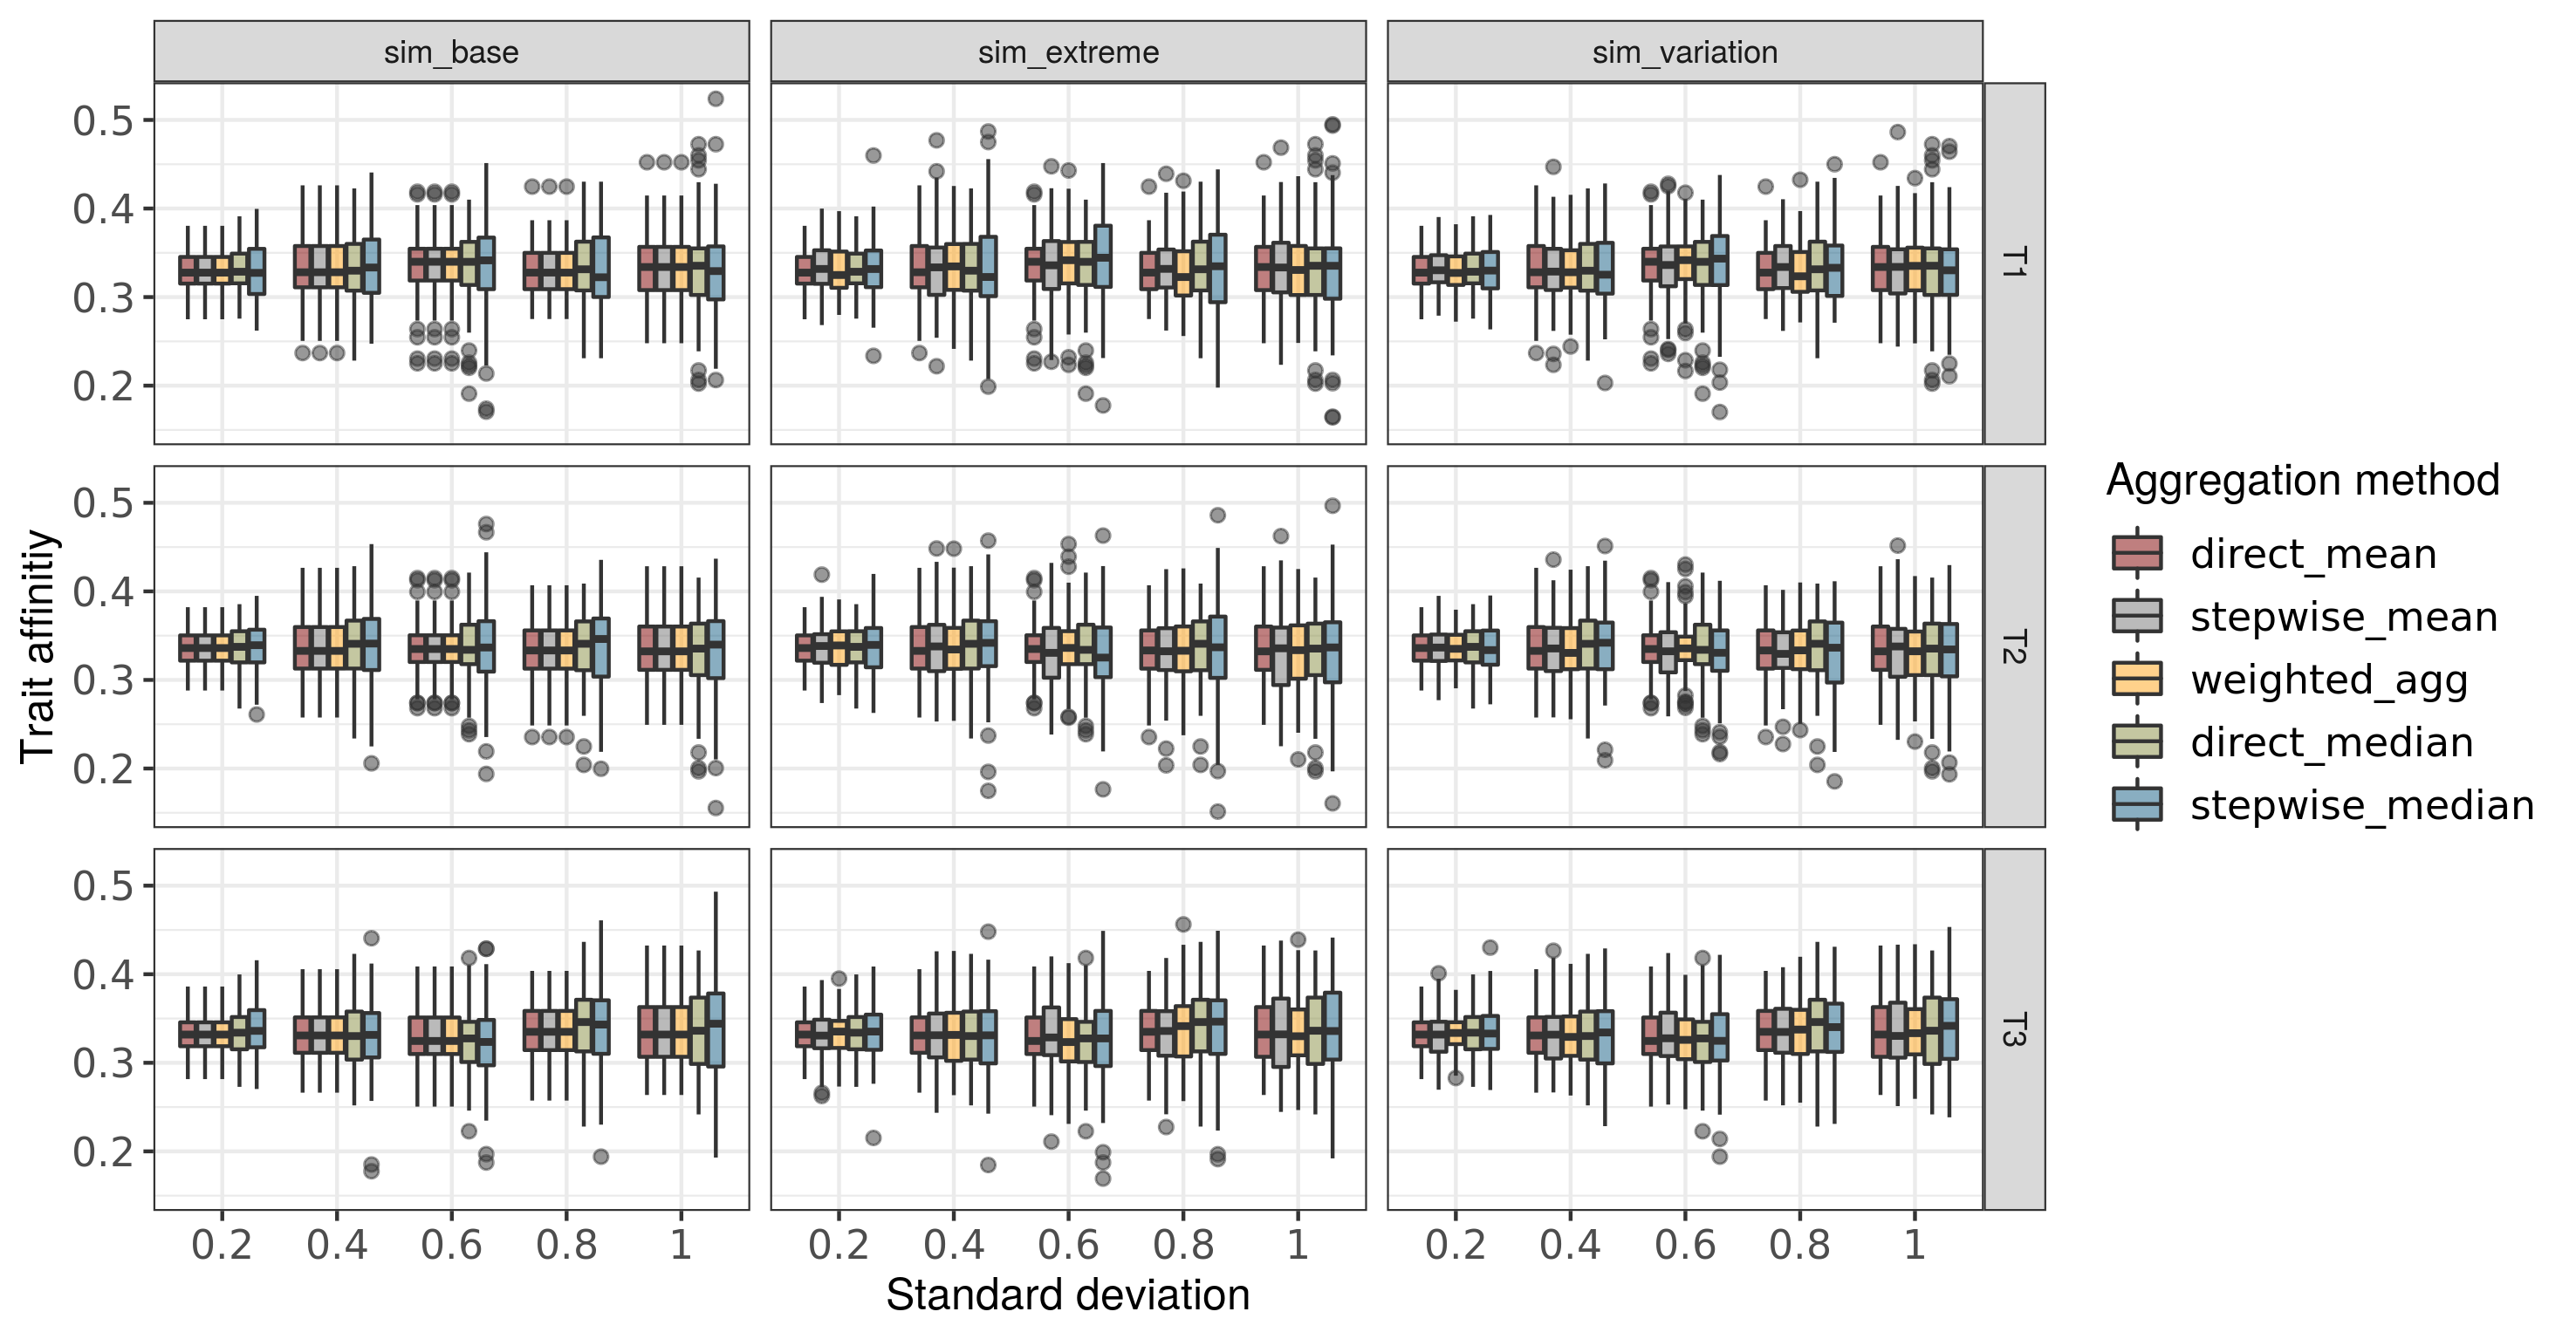
\includegraphics[width=16.5cm, height=10cm]{Overview_sim_results.png}
  \caption{Ranges of aggregated trait affinities for the three examples of taxonomic hierarchies and simulated levels of trait variability. Boxplots depict results for each trait aggregation method of 100 simulations. T1, T2, and T3 are the simulated traits.}
  \label{fig:overview_sim_results}
\end{figure}

\begin{figure}[H]
  \centering
  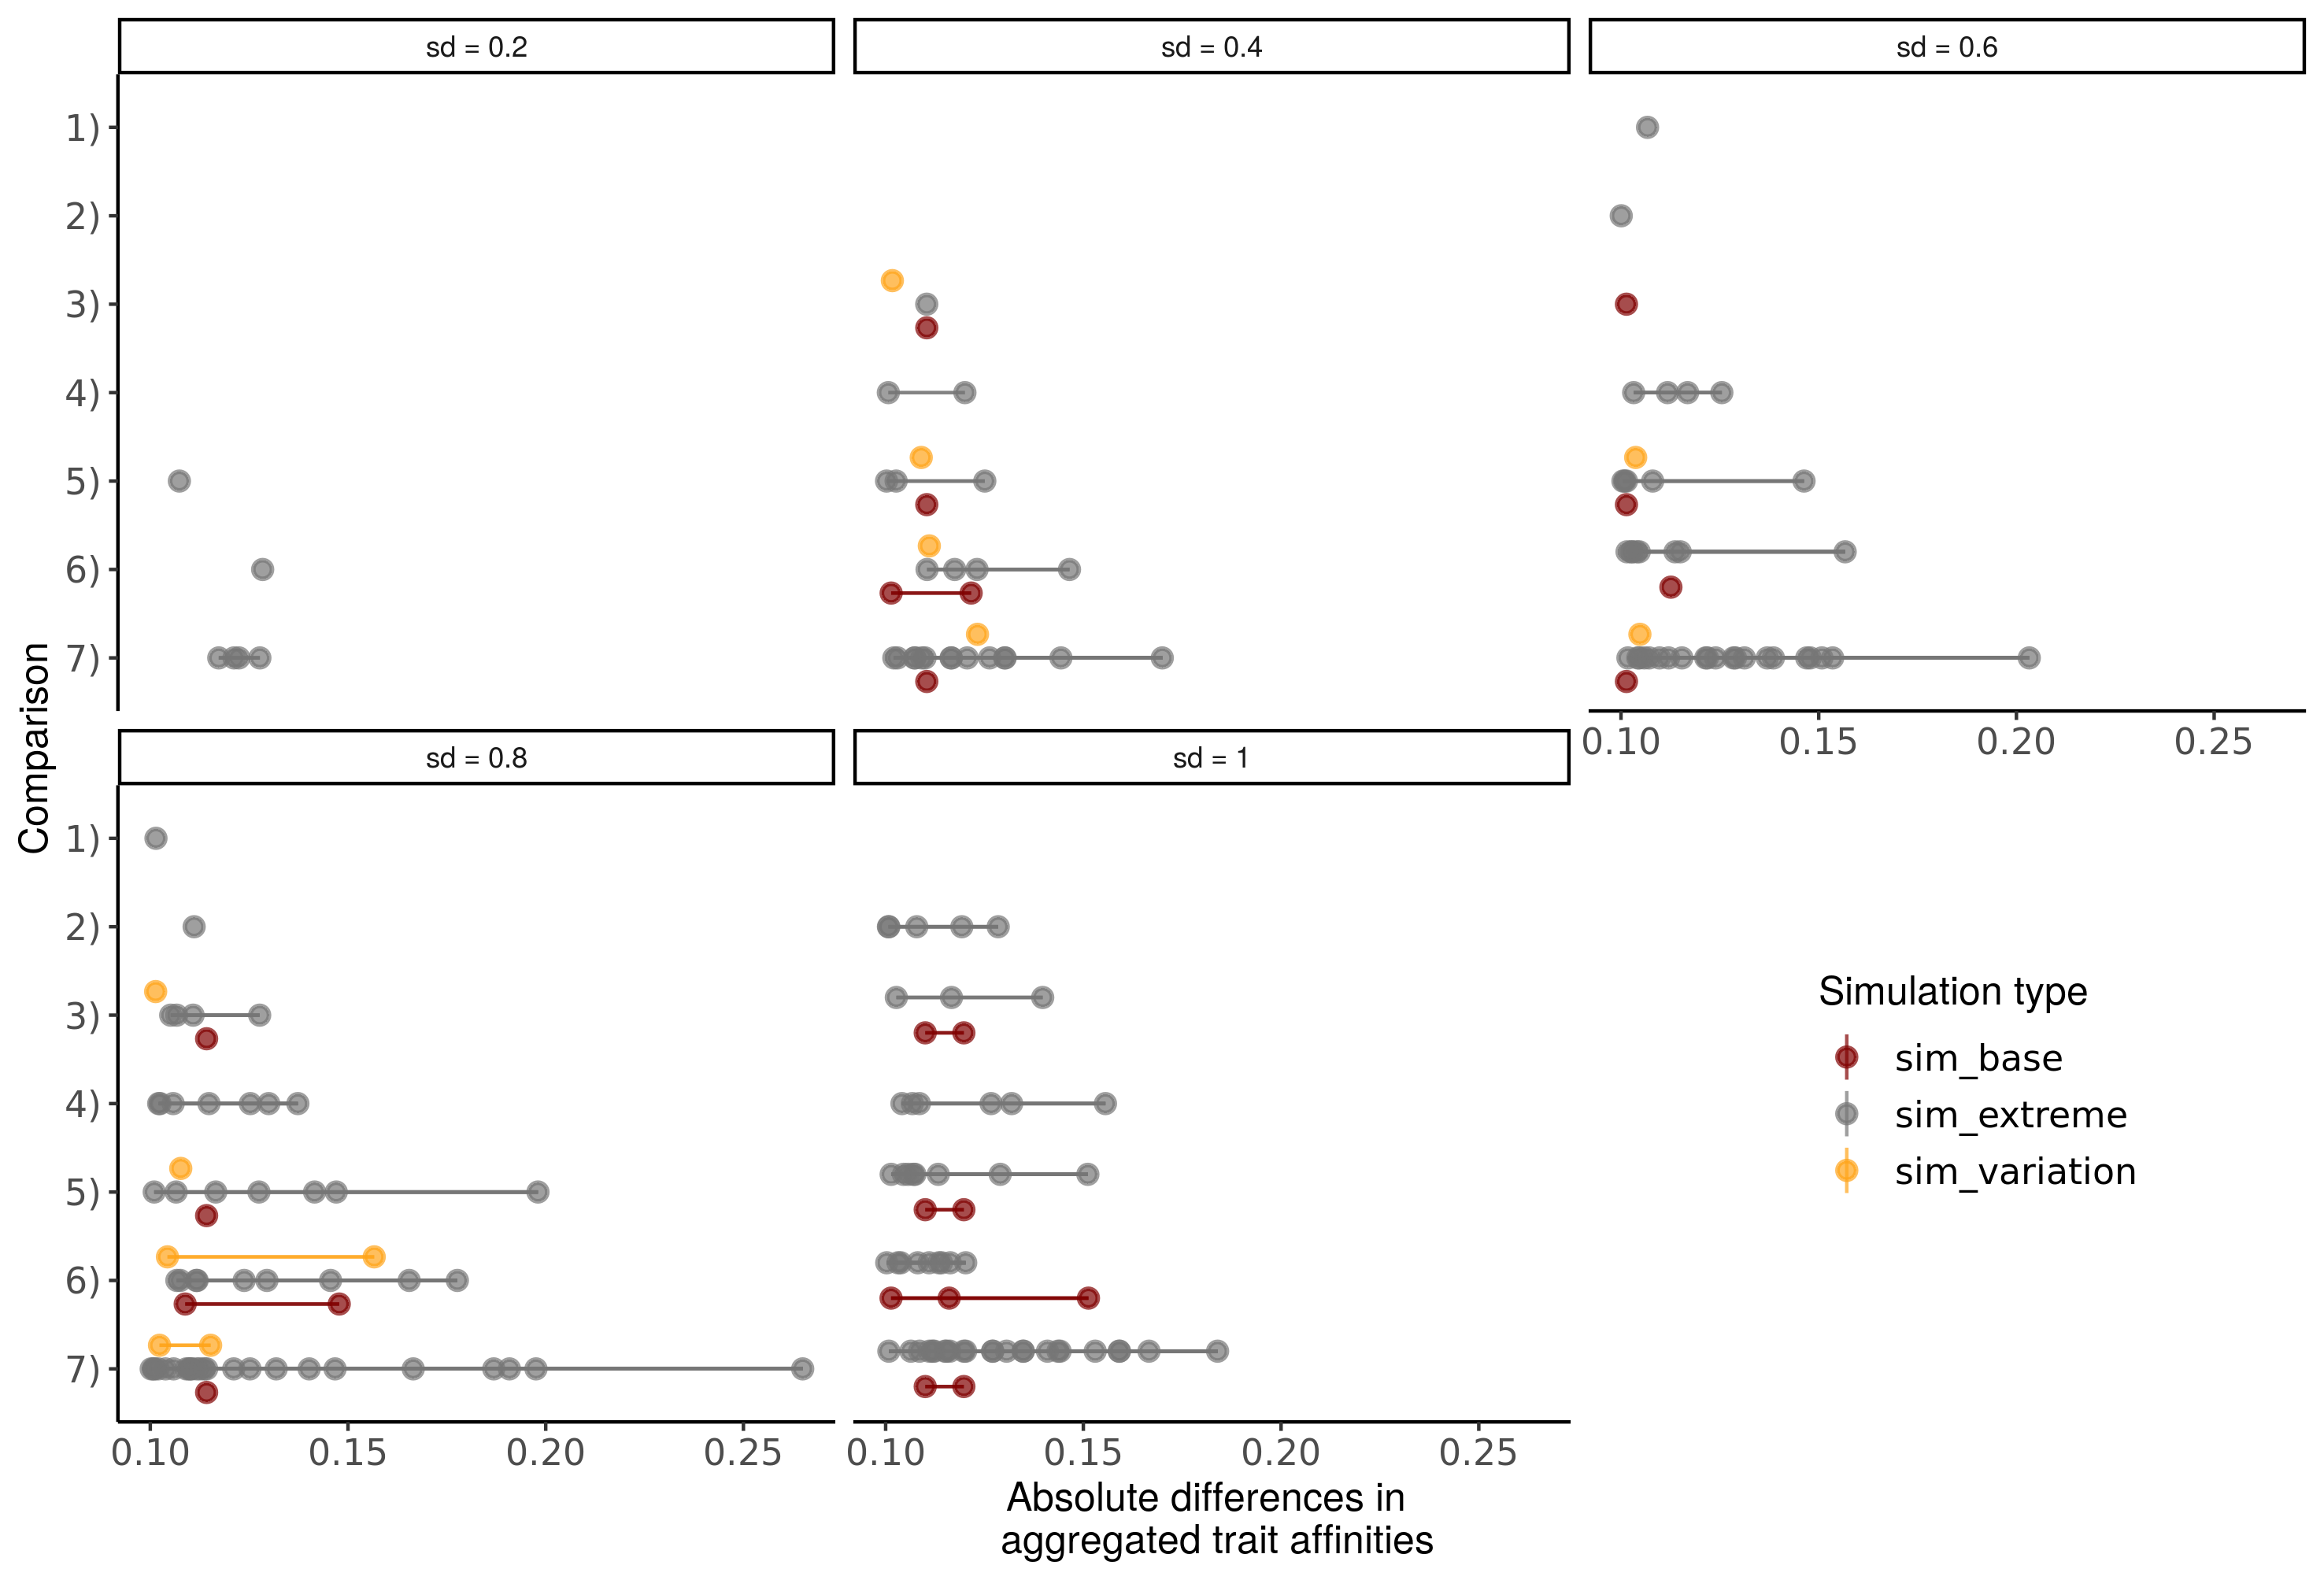
\includegraphics[width=16.5cm, height=10cm]{Diffs_indiv_runs_sim.png}
  \caption{Comparison of the aggregated trait affinities produced by the different trait aggregation methods for every simulated dataset across all 3 simulated traits. Dots depict comparisons where absolute differences between aggregated trait affinities were greater than 0.1. \newline
  Comparison: \newline
  1) Direct\_agg (median) - Stepwise\_agg (mean) \newline
  2) Direct\_agg (median) - Weighted\_agg, \newline
  3) Stepwise\_agg (mean) - Stepwise\_agg (median), \newline
  4) Stepwise\_agg (mean) - Weighted\_agg, \newline  
  5) Direct\_agg (mean) - Stepwise\_agg (median), \newline
  6) Direct\_agg (median) - Stepwise\_agg (median), \newline
  7) Stepwise\_agg (median) - Weighted\_agg \newline
  }
  \label{fig:sim_indv_runs}
\end{figure}

\newpage

\subsection*{Differences in trait affinities obtained by trait aggregation methods compared to traits assigned at family-level}
\label{sec:diff_trait_agg_chessman}

The percentage of differing cases of trait affinities obtained by the trait aggregation methods compared to trait affinities originally assigned at family-level varied between 16.2 \% and 22.9 \% for the Australian dataset. For the North American dataset, comparison of the trait aggregation methods to trait affinities assigned at family-level yielded between 15.3 \% and 47 \% differing cases (Table \ref{tab:summary_stat_aggr_vs_fam_assigned}). In general, trait aggregation methods using the median yielded fewer cases with differences compared to approaches using the mean. However, aggregation methods using the median produced greater differences for both datasets. Standard deviations of absolute differences were similar for all tested aggregation methods. For both datasets maximum differences of 1 occurred for all investigated grouping features (Figure \ref{fig:diff_aggr_traits_chessman} and Figure \ref{fig:diff_aggr_traits_pyne}).

% Is that necessary?
A comparison of the aggregation methods with each other for the 4 datasets revealed that differences in aggregated trait affinities were largest between the \textit{stepwise\_agg\textsubscript{median}} and \textit{direct\_agg\textsubscript{median}} (Figure \ref{fig:comp_aggr_methods}).

\begin{table}[H]
  \centering
  \caption{Amount of differing cases, the minimum and maximum, and means and standard deviations of absolute differences between trait affinities assigned at family-level and aggregated trait affinities.}
  \label{tab:summary_stat_aggr_vs_fam_assigned}
  \begin{tabular}{ll|ccccc}
  \toprule[.1em]
  Database & \specialcell{Comparison to\\ traits at fam.-lvl.} & \specialcell{Differing \\ cases [\%]} & \specialcell{Min. \\ differences} & \specialcell{Max. \\ differences} & \specialcell{Mean abs. \\ differences} & \specialcell{SD abs. \\ differences} \\ 
  \toprule[.1em]
  \multirow{4}{*}{\specialcell{Australia \\ (Chessman)}} & \specialcell{direct\_agg (median)} & 16.53 & 0.01 & 1.00 & 0.45 & 0.27 \\ 
  & \specialcell{direct\_agg (mean)} & 23.24 & $< 0.01$ & 0.99 & 0.34 & 0.23 \\ 
  & \specialcell{stepwise\_agg (median)} & 17.90 & 0.01 & 1.00 & 0.42 & 0.26 \\ 
  & \specialcell{stepwise\_agg (mean)} & 23.24 & $< 0.01$ & 0.99 & 0.33 & 0.22 \\ 
  & \specialcell{weighted\_agg} & 23.24 & $< 0.01$ & 1.00 & 0.34 & 0.24 \\ 
  \midrule
  \multirow{4}{*}{\specialcell{North America}} & \specialcell{direct\_agg (median)} & 15.33 & 0.17 & 1.00 & 0.70 & 0.26 \\ 
  & \specialcell{direct\_agg (mean)} & 47.00 & $< 0.01$ & 1.00 & 0.30 & 0.26 \\ 
  & \specialcell{stepwise\_agg (median)} & 18.00 & 0.08 & 1.00 & 0.63 & 0.28 \\ 
  & \specialcell{stepwise\_agg (mean)} & 47.00 & $< 0.01$ & 1.00 & 0.30 & 0.27 \\ 
  & \specialcell{weighted\_agg} & 47.00 & $< 0.01$ & 1.00 & 0.31 & 0.28 \\ 
  \bottomrule
  \end{tabular}
\end{table}

\newpage

\begin{figure}[H]
  \centering
  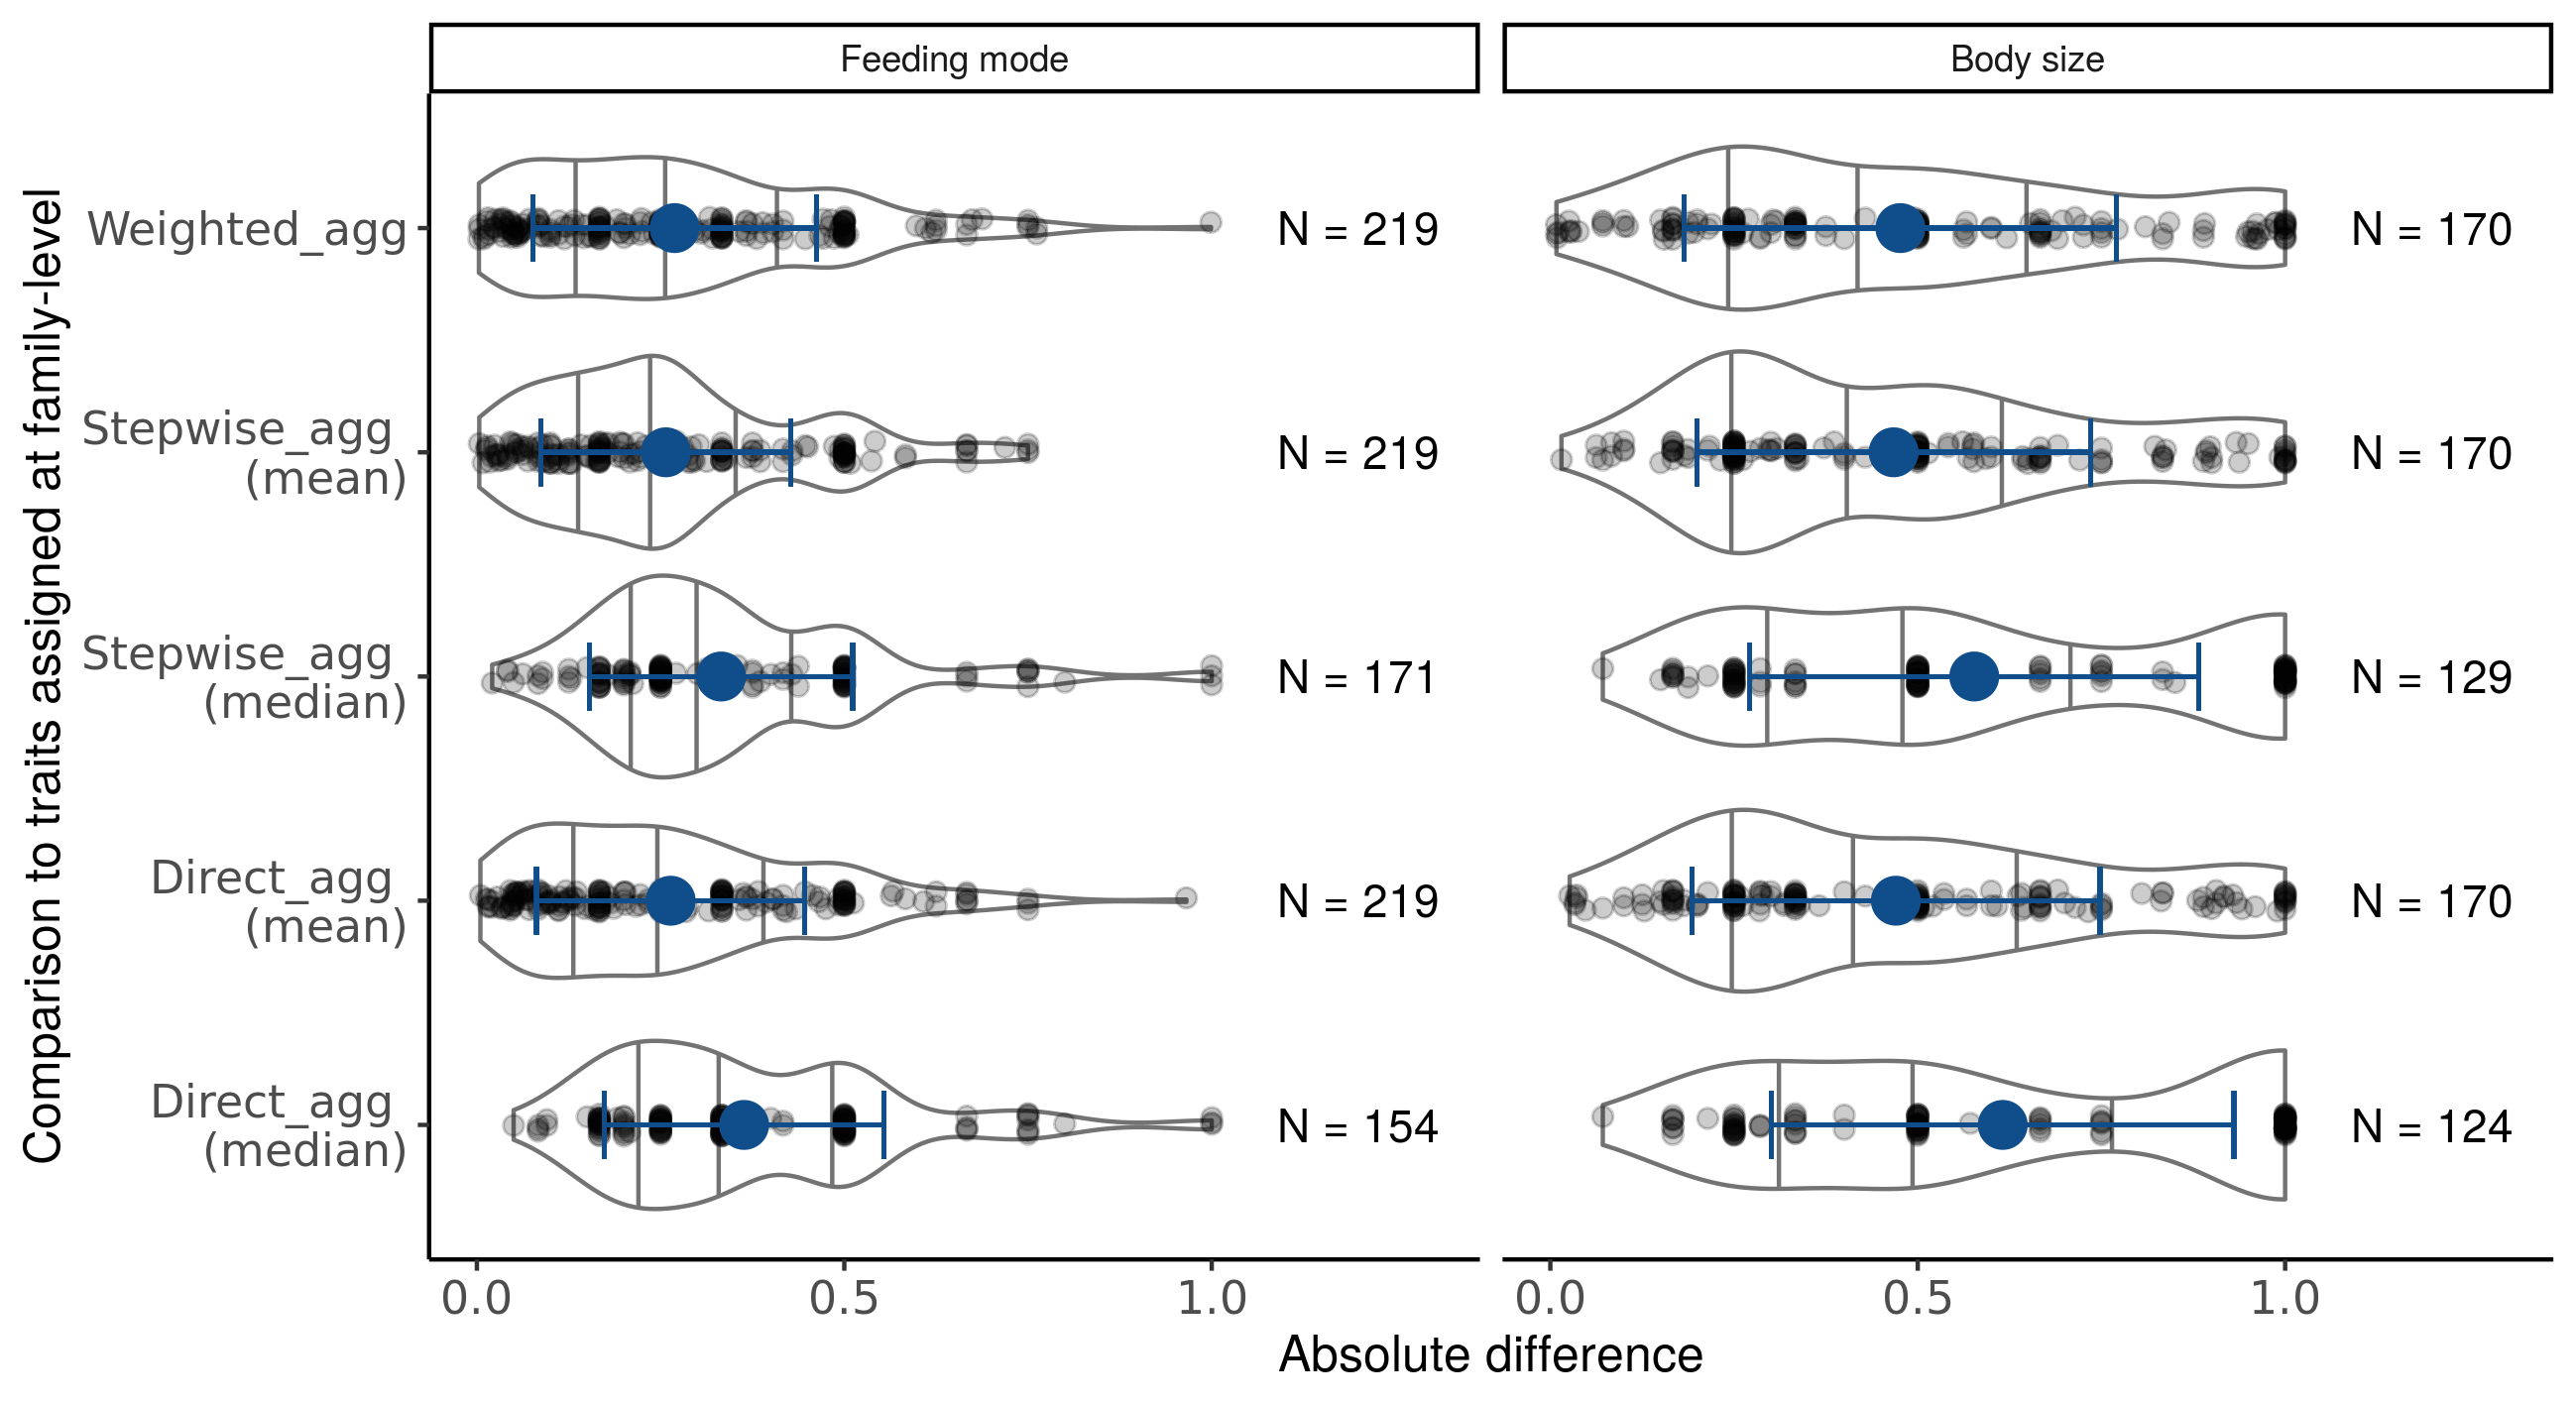
\includegraphics[width=16.5cm, height=10cm]{Deviances_trait_agg_chessman.png}
  \caption{Display of the cases (factor combination investigated families and traits) where differences occurred between aggregated traits and traits assigned at family-level. Violin plots - a mirrored density plot - show the density of the absolute trait affinity differences for the Australian dataset for the grouping features feeding mode and body size. Absolute differences in trait affinities are depicted as gray dots. N denotes the number of cases per comparison where differences occurred. The blue dot indicates the mean of absolute differences and the error bars the standard deviation. The gray vertical lines show the 25th, 50th and 75th quantile of the density estimate.}
  \label{fig:diff_aggr_traits_chessman}
\end{figure}


\begin{figure}[H]
  \centering
  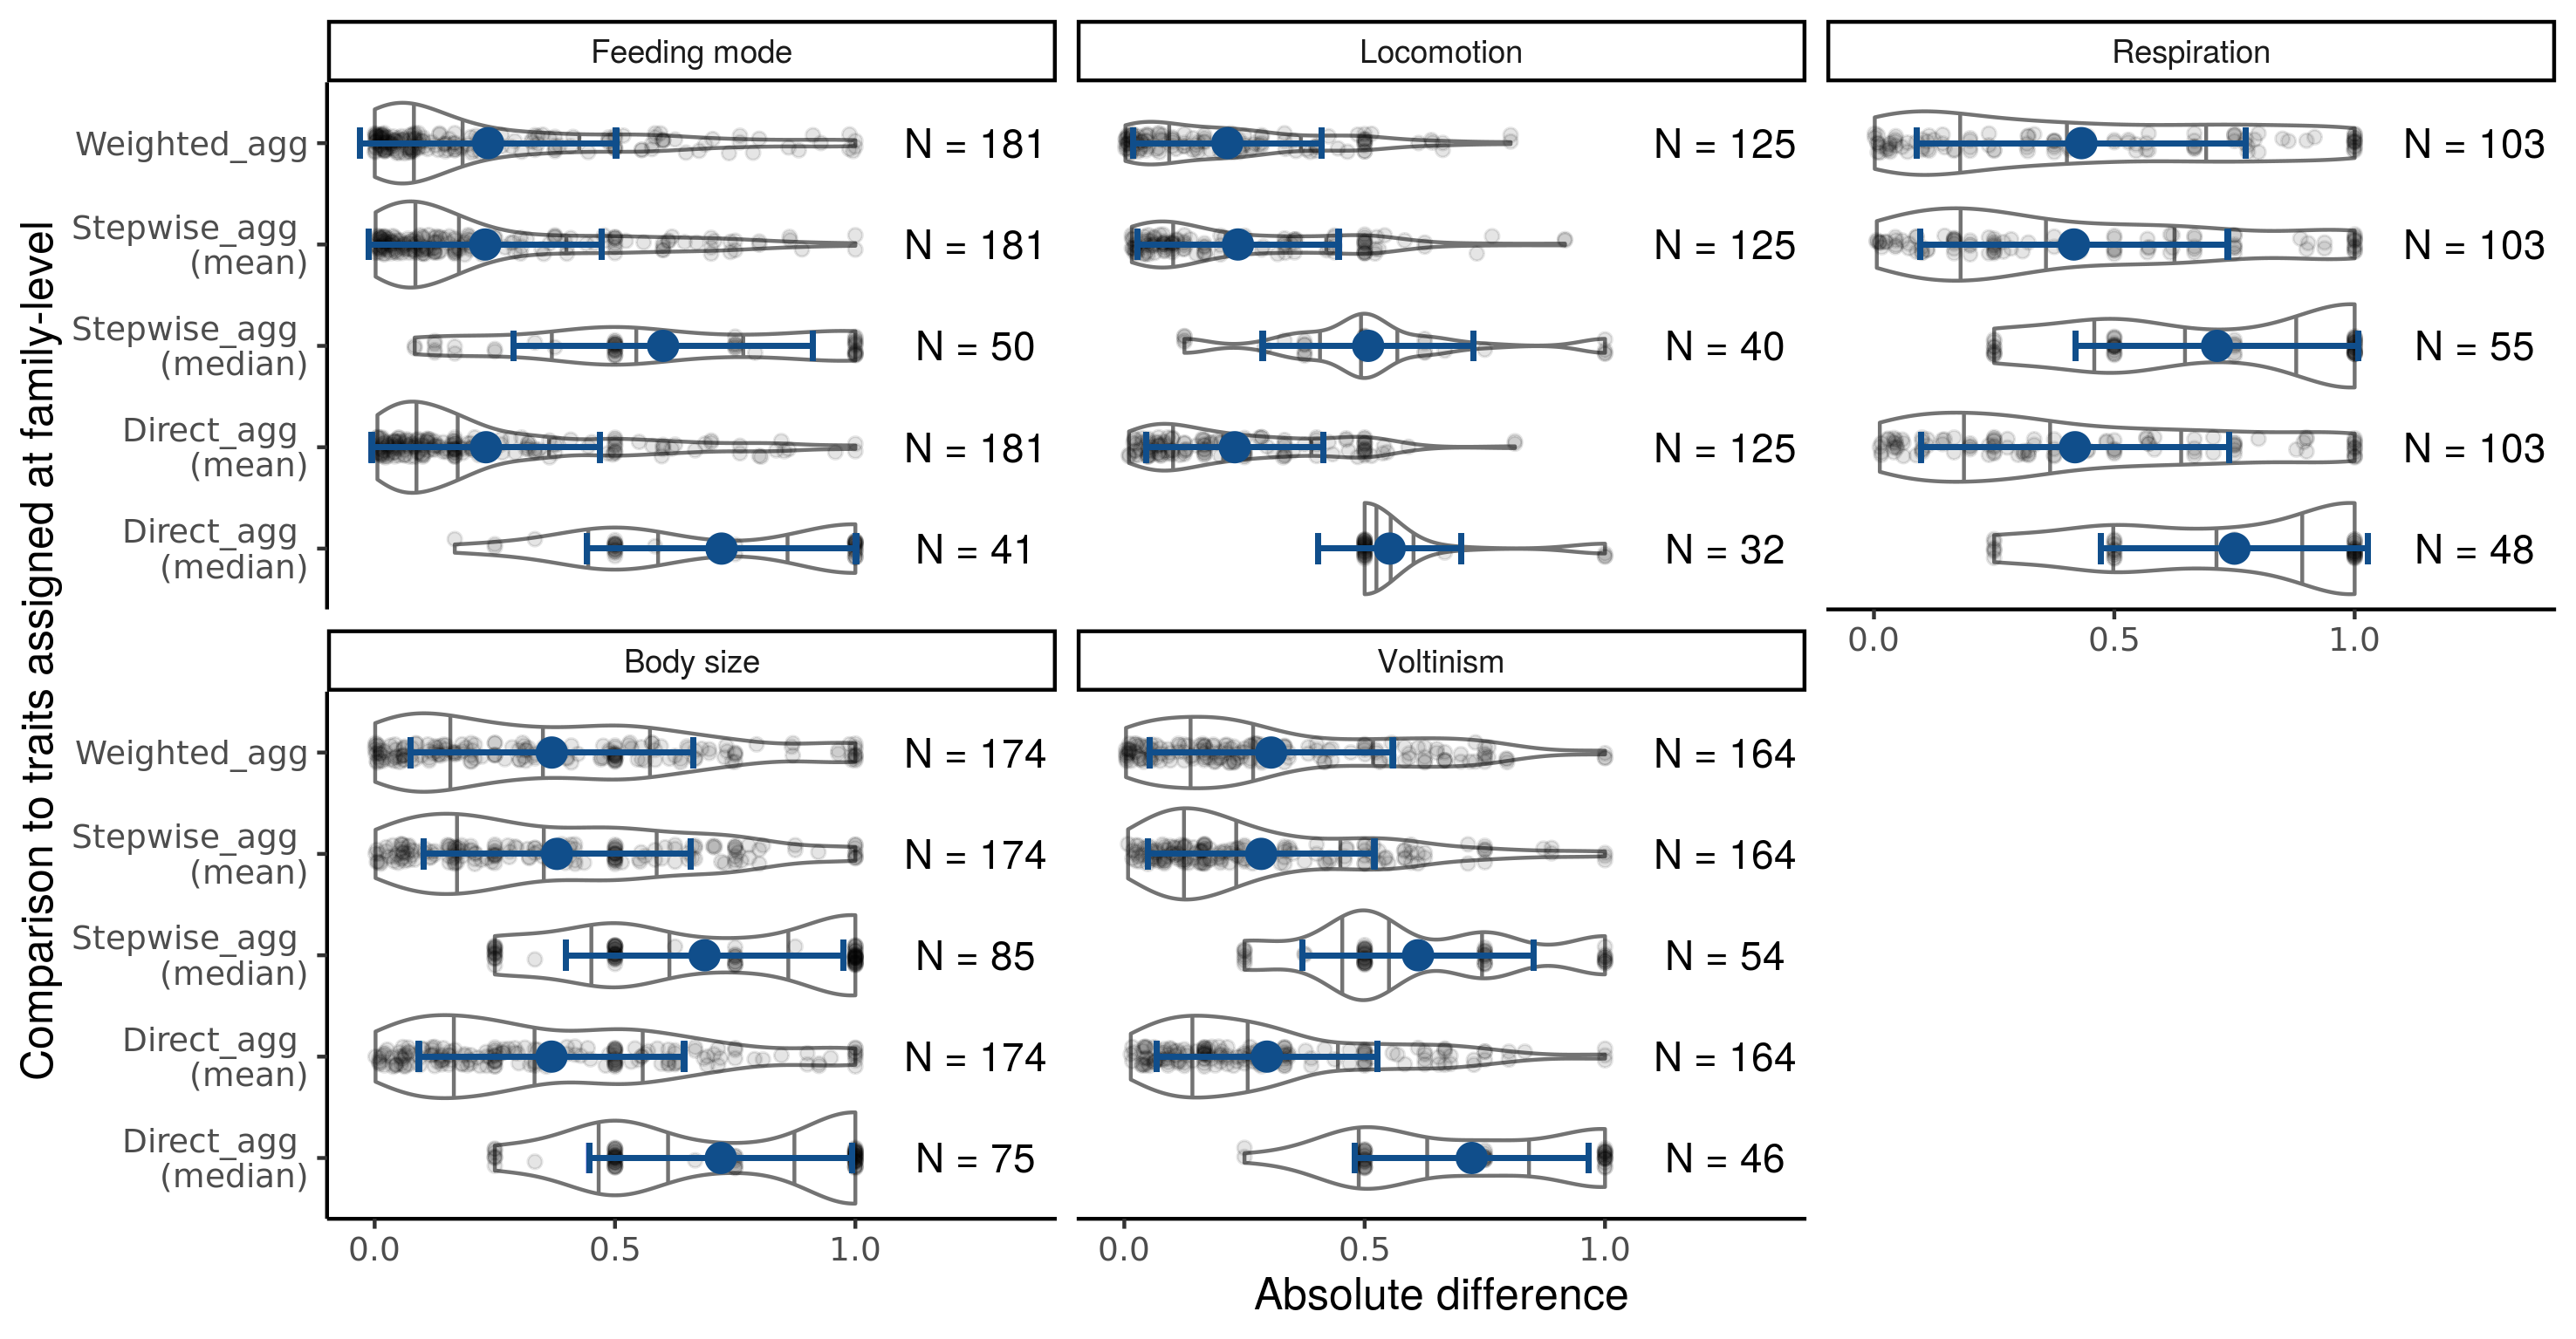
\includegraphics[width=16.5cm, height=10cm]{Deviances_trait_agg_pyne.png}
  \caption{Display of the cases (factor combination investigated families and traits) where differences occurred between aggregated traits and traits assigned at family-level. Violin plots - a mirrored density plot - show the density of the absolute trait affinity differences for the North America dataset for the grouping features feeding mode, locomotion, respiration, body size and voltinism. Absolute differences in trait affinities are depicted as gray dots. N denotes the number of cases per comparison where differences occurred. The blue dot indicates the mean of absolute differences and the error bars the standard deviation. The gray vertical lines show the 25th, 50th and 75th quantile of the density estimate.}
  \label{fig:diff_aggr_traits_pyne}
\end{figure}

\newpage 

%%%%%%%%%%%%%%%%%%%%%%%%%%%%%%%%%%%%%%%%%%%%%%%%%%%%%%%%%%%%%%%%%%%%%%%%%%%%%%%%%%%%%%%%%%%%%%%%%%%%

\subsection*{Re-analysis of Szöcs et al. using harmonised and aggregated grouping features}

The original RDA in Szöcs et al. \cite{szocs_effects_2014} indicated that downstream sites (high salinity) were characterised by the traits shredder, ovoviviparity, multivoltinism, long life cycle duration ($> 1$ year), and gill respiration and upstream sites (low salinity) were characterized by univoltinism, oviposition in clutches and short life cycle duration ($< 1$ year). 

Using harmonised grouping features resulted in less traits that distinguish upstream and downstream sites in comparison to the original analysis (Figure \ref{fig:rda_species_scores} and Figure \ref{fig:boxplots_scores_on_constrained_axis}). According to the RDA of the trait composition, downstream sites were characterised by taxa with the traits multivoltinism, ovoviviparity and long life cycle duration. Upstream sites were characterised by univoltine taxa with a short life cycle duration that lay their eggs in an aquatic environment (aquatic eggs). The trait aquatic eggs of the harmonised grouping feature oviposition has been derived by amalgamating the trait oviposition in clutches and other related traits (Table \ref{tab:traits_harmonization}). The traits shredder and gill respiration did not characterise sites with high salinisation.

Using at family-level aggregated traits from the harmonised dataset showed also results similar to the original analysis but with fewer traits distinguishing upstream and downstream sites (Figure \ref{fig:rda_species_scores} and Figure \ref{fig:boxplots_scores_on_constrained_axis}). The \textit{direct\_agg\textsubscript{mean}}, \textit{direct\_agg\textsubscript{median}}, and \textit{weighted\_agg} 
characterised the downstream sites with the same traits as the original analysis except that downstream sites were not characterised by the trait shredder. Upstream sites were characterised by the traits univoltinism, aquatic eggs and short life cycle duration. The same results were obtained when re-analysing the data with traits aggregated by the \textit{stepwise\_agg\textsubscript{mean}} and \textit{stepwise\_agg\textsubscript{median}}, with the exception that none of the life cycle traits characterised upstream or downstream sites. Thus, in our comparison aggregating by \textit{direct\_agg\textsubscript{mean}}, \textit{direct\_agg\textsubscript{median}}, and \textit{weighted\_agg} yielded to the least change in interpretation of the RDA results compared to the original results.

\begin{figure}[H]
    \label{fig:rda_species_scores}
    \centering
    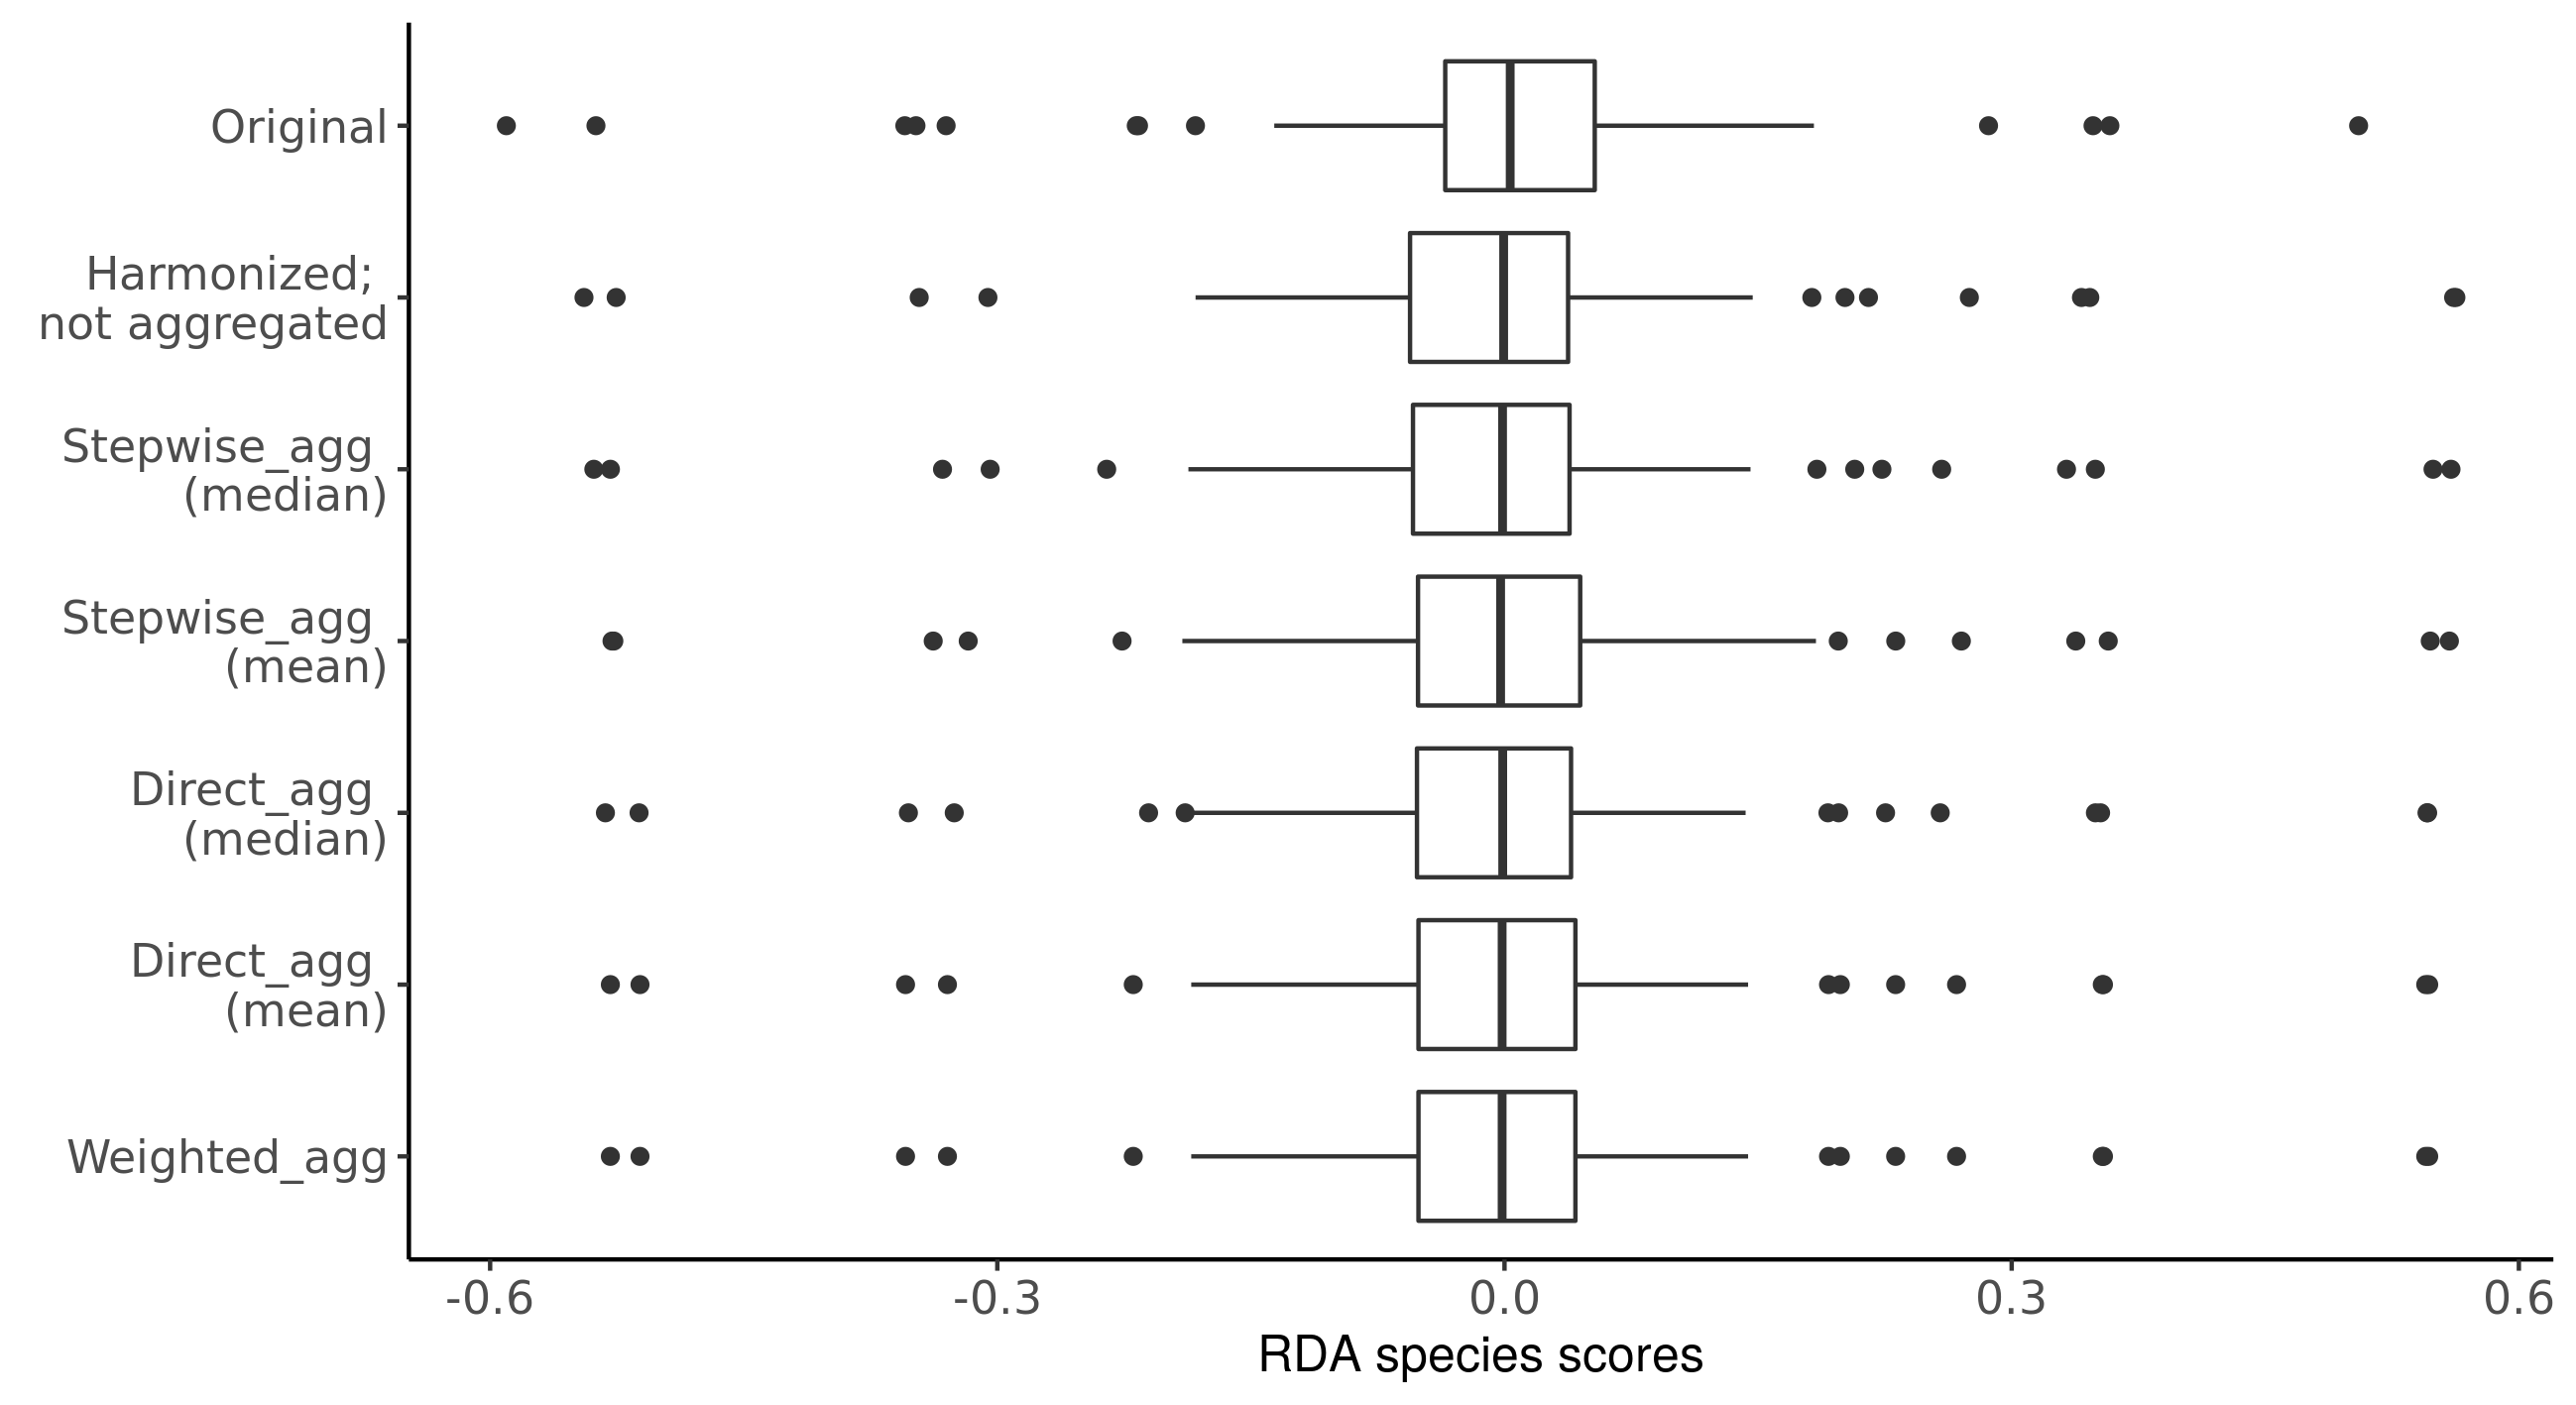
\includegraphics[width=16.5cm, height=10cm]{Species_scores_rda.png}
    \caption{Species scores obtained by RDA from the original analysis \cite{szocs_effects_2014}, using harmonised grouping features, and using harmonised grouping features with traits aggregated to family-level. The dots represent the individual species scores for each analysed trait along the conductivity axis. The violin plot shows the density estimate of the species scores. Gray vertical lines indicate the median of the obtained species scores.}
\end{figure}

\begin{sidewaysfigure}
  \label{fig:boxplots_scores_on_constrained_axis}
  \centering
  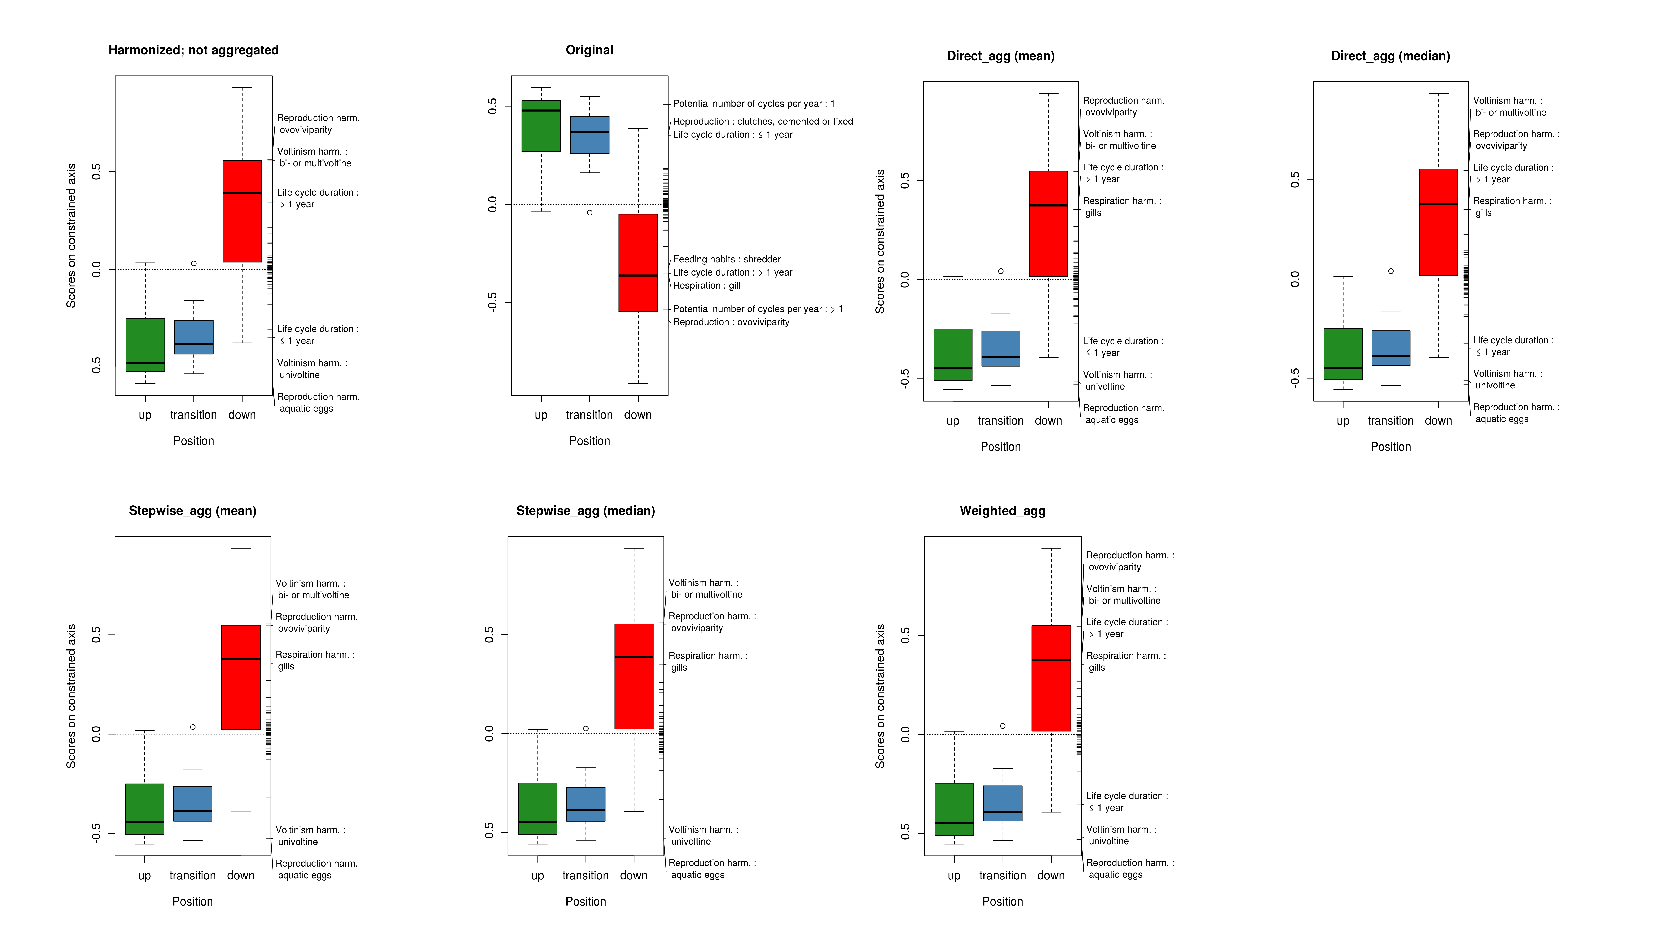
\includegraphics[width= 22cm, height=12cm]{Scores_on_constrained_axis_combined.pdf}
  \caption{RDA of traits constrained by electric conductivity for the tested methods and the original study. Shown are boxplots of the site scores along the conductivity axis. The rug on the right side of each plot indicates species scores of the traits on the conductivity axis. Only traits with a mahalanobis distance greater than the $97.5 \%$ quantile of the Chi-square distribution (5.02) were labelled.}
\end{sidewaysfigure}

\newpage

%%%%%%%%%%%%%%%%%%%%%%%%%%%%%%%%%%%%%%%%%%%%%%%%%%%%%%%%%%%%%%%%%%%%%%%%%%%%%%%%%%%%%%%%%%%%%%%%%%%%

\section*{Discussion}

% 1. Allgemeiner Satz zum Thema, der auf eine offene Frage o.ä. hinweist
% 2. Was haben wir herausgefunden?
% 3. Was haben andere schon herausgefunden
% 4. Was bedeutet das für zukünftige Studien?

% 1. Trait Database 
%- Unterschiede zwischen Regionen und Trait Genauigkeit
%- Was kann man machen
%- Andere Studien zur Trait Harmonisierung usw.

\subsection*{Trait definition discrepancies and taxonomic resolution}

% Why do we need trait-based analysis, especially across regions?
Synthesizing trait information from multiple trait databases is crucial to unfold the full potential of trait-based approaches, e.g. for studying community trait responses to environmental gradients worldwide. Our attempt of harmonising invertebrate trait information from trait databases of different regions showed that grouping feature harmonisation is labour-intensive because grouping features are differentiated differently into traits between trait databases and various codings are used to describe traits. In addition, the same traits are sometimes defined differently in the investigated databases, requiring expert knowledge to reclassify these traits (e.g. the trait piercer in the Tachet database, Table \ref{tab:traits_harmonization}). Although, others have noted the lack of standardised trait terminology in freshwater ecology \cite{baird_toward_2011, brink_traits-based_2011} we are the first to describe invertebrate trait definition discrepancies for some commonly used grouping features.
%In addition we provide harmonised grouping feature trait datasets that can be used for other studies
To resolve definition discrepancies and facilitate data synthesis in the future terminological standards are needed. Harmonised definitions and concepts of traits have been developed in the past for other organism groups, e.g. for plants with the \textit{Thesaurus Of Plant characteristics} (TOP) initiative \cite{garnier_towards_2017}. The core of this harmonisation initiative is to provide standardised trait definitions and to draw connections to synonyms, related terms, and surrounding concepts by linking to other controlled vocabularies or ontologies in the field. Such initiatives could be a role model for freshwater ecologists to establish unambiguous terminologies for invertebrate traits. The existing freshwater invertebrate trait databases could be linked through standardised terminologies or ontologies, as suggested by Baird et al. \cite{baird_toward_2011} almost a decade ago. By following the recently proposed \textit{Ecological Trait-data Standard Vocabulary} (ETS) providers of invertebrate trait data could connect their traits to such ontologies \cite{schneider_towards_2019}. Once standardised trait definitions are established, these will improve trait data sharing, trait data processing when working with multiple trait databases, and ultimately interpretation of the derived results. % What is not mentioned here is how traits are measured, for which measurement protocols exist I believe. I think this is an separate issue. 

% ?What's the problem with the state of data coverage
Our analysis aimed to use most of the available invertebrate trait information for different regions to establish harmonised grouping feature datasets. Although many taxa are covered in the trait databases from which we extracted our trait datasets, the availability of trait information varies strongly across grouping features and taxonomic resolution differs between databases. While trait information from Europe and New Zealand was mainly on species-level, considerable portions of trait data from North America and Australia were on genus or family-level (Table \ref{tab:tax_coverage}). Assigned traits on family-level might not reflect the real trait diversity within a taxon, for example for Chironomidae \cite{serra_synthesising_2016}. However, species identification can be complicated and time-consuming \cite{marshall_taxonomic_2006, resh_which_2008}, and therefore trait information on family-level has been widely used, e.g. in bioassessment \cite{beketov_spear_2009}.
% How would obtaining information on species level change our results?

% Include Ben's point?
% Discussion point BK: It is intersting that Australia has fewer species and genus than NOA and EU (not suprisngly since the datasets in Oz were mostly delveoped at family level) but more families than these other regions. I wonder if this indicates that Family richness is really higher in Australia. Perhaps it might be as Australia has a wider range of evolutionary histories. This would be worth considering in the discussion  


%%%%%%%%%%%%%%%%%%%%%%%%%%%%%%%%%%%%%%%%%%%%%%%%%%%%%%%%%%%%%%%%%%%%%%%%%%%%%%%%%%%%%%%%%%%%%%%%%%%%%%
% 2. + 3. die aktuellen Abschnitte (obwohl sie auch etwas ähnliche Themen beinhalten - geht ja immer um was ähnliches - wie gut sind die Aggregationsmethoden - könnte man vielleicht auch zusammenfassen
% Hier: Überschrift mit genereller Aussage?

\subsection*{Trait aggregation}

% Why is it important to investigate trait aggregation methods? And trait harmonisation?
When trait values are only available at species-level and observational data are on less precise taxonomic levels various trait aggregation methods have been used by researchers. We aggregated traits from an Australian and North American trait dataset to family-level using 5 different aggregation methods and compared the results to traits assigned at family-level for these regions. Evaluation of the differences between aggregated and assigned traits is difficult because it remains unclear what the true value of a particular trait for a particular family is. Aggregation of trait information on species or genus-level to a point estimate on family-level suggests a precision which is not necessarily present, especially not for traits with a high variability or if trait information on species-level is missing. Some traits can vary strongly on more precise taxonomic levels than the family-level. For example, Monaghan and Soares \cite{monaghan_improving_2013} found a high intra-family trait dispersion in the Tachet database for traits of the grouping features body size, flow preference, and reproduction. Furthermore, studies focusing on the lability of traits, i.e. how much traits are unconstrained by phylogeny, found that traits of ecological preferences (e.g. thermal preference), body size, resistance forms, and to a lesser extent feeding mode are labile, and thus possibly highly variable \cite{poff_functional_2006, wilkes_traitbased_2020}. However, if trait aggregation is necessary our study can give guidance, under which circumstances the choice of aggregation method might be important. The 5 aggregation methods we tested use either the mean or the median and different weightings. Our results indicated that 1) the aggregation methods \textit{direct\_agg\textsubscript{median}} and \textit{stepwise\_agg\textsubscript{mean}} (median aggregation methods) compared to \textit{direct\_agg\textsubscript{mean}}, \textit{stepwise\_agg\textsubscript{mean}}, and \textit{weighted\_mean} (mean aggregation methods) were often closer to the assigned traits at family-level and 2) that the different weightings tested exerted a minor impact on the aggregated trait affinities. We obtained for both datasets more differing cases for mean aggregation methods, irrespective of the weighting. In the Australian dataset, the amount of differing cases was slightly higher for the mean aggregation methods (23 \%) than for median aggregation methods (16 to 18 \% differing cases). In the North American dataset, mean aggregation methods yielded in 47 \% of the cases a difference to the assigned traits, much higher in comparison to the median aggregation methods (between 15 and 18 \%, Table \ref{tab:summary_stat_aggr_vs_fam_assigned}). When differences occurred between median aggregation methods and assigned traits, these differences were greater compared to the mean aggregation methods, particularly for the North American dataset. There, the mean absolute differences for the median aggregations was twice as high (0.63 - 0.7) compared to the mean aggregations (0.3 - 0.31, Table \ref{tab:summary_stat_aggr_vs_fam_assigned}). The differences can be explained by the binary coding used in the North American trait dataset and in the assigned traits. As a result, traits have affinities of either 1 or 0. Therefore, traits of a particular grouping feature have in most cases a higher difference in trait affinities to each other than if they were fuzzy coded. Using the median to aggregate binary coded taxa will often result in a value of 0 or 1, while using the mean will often result in values between 0 and 1. 
% Was folgt daraus?
%Thus, using the median led for the North American dataset in many cases to agreement with the assigned traits. However, when differences were found the difference between median aggregated traits and assigned traits was often 1. 
% except for traits were binary coding was not mutually exclusive and when same number of 0 and 1

The weightings explored in this analysis should lead to different aggregated trait affinities in cases where genera within a family have different numbers of species. In fact, the simulation results indicated that for a particular family where one genus has a much larger number of species compared to the other genera, weighting the number of taxa can lead to different aggregated trait affinities, sspecially for traits with higher levels of variance (Figure \ref{fig:sim_indv_runs}. However, in the comparison of the trait aggregation methods to assigned traits the number of differing cases and the mean absolute differences in trait affinities were similar across the mean aggregation and across the median aggregation methods, which suggests a small influence of the weightings on the aggregation methods. Also, the distributions of absolute trait affinity differences to assigned traits were relatively similar for the mean aggregation methods and the median aggregation methods respectively (Figure \ref{fig:diff_aggr_traits_chessman} and Figure \ref{fig:diff_aggr_traits_pyne}). The minor impact on trait aggregation of the weightings may be explained by the fact that a considerable portion of taxa had low numbers of genera or species entries. From the taxa that were compared from the North American trait dataset, 14 \% were resolved on family-level and 62 \% were resolved on genus-level. 52 \% had 5 or less genera and 13 \% contained just one genus (Figure \ref{fig:tax_hierarchy_NOA}). In the Australian dataset, 21 \% of the taxa were resolved on family-level, 40 \% were resolved on genus level, and 39 \% were resolved on species-level. 68 \% of the taxa contain 5 or less genera and 40 \% just contained one genus (Figure \ref{fig:tax_hierarchy_AUS}). Hence, these results are expected to change when trait information is all on species level 

\subsection*{Grouping feature harmonisation}

We explored how using harmonised grouping features and aggregated traits might change the results of trait-environment relationships. We are not aware of other studies that compared trait-environment relationships using harmonised and not harmonised data. The re-analysis yielded only slightly different results compared to the original study, i.e. some of the traits that responded in the original analysis did not respond in the re-analysis. Those traits that were non-responsive in the re-analysis were those closest to the criterion that defined when a trait was associated with either high or low salinity (mahalanobis distance greater than the 97.5 \% quantile of the Chi-square distribution, see method section), namely feeding mode shredder, respiration gills, and life cycle duration traits. Feeding mode shredder was the only trait that was non-responsive when using harmonised (but not aggregated) as well as when using aggregated data. One reason for the non-responsiveness of shredders in the re-analysis was likely the harmonisation procedure. For example, during harmonisation the trait shredder has been amalgamated based on three traits (Miner, xylophagus, and shredder). As a result, the trait affinities in the original data have a higher mean and standard deviation than in the aggregated and harmonised data (Table \ref{tab:SI_resp_traits_summary_stats}) suggesting that the signal in the original data has presumably been weakened by the harmonisation. This might be the reason that shredders showed a less strong reaction to the salinity gradient in the re-analysis. These findings show that if harmonisation is necessary, harmonised and non-harmonised data, if available, should be compared and possible averaging effects should be considered in further analysis. The fact that the family-level aggregated traits used in the re-analysis showed only slightly different results compared to the original analysis is in line with the findings of others that family-level traits can be sensitive enough to detect environmental impacts \cite{beketov_spear_2009}.
% Although species-level traits are expected to result in more precise results when investigating trait-environment relationships. % Cite Schmidt Kloiber? Cite another paper that uses family-level trait data

% Keep it simple!
% Resp gills: Original data has a lot of zeros, which are not present in the harmonised \& aggregated datasets (see % In the analysis with the harmonised dataset resp gills is not responding to the salinity gradient
% Aggregated data look similar to the harmonised ones, but resp gills is here one of the traits responding to conductivity!
% Why did some aggregated datasets promote life cycle duration traits and others not
% Results using trait data obtained when aggregating with stepwise\_agg (median) and stepwise\_agg (mean) indicate that life cycle duration traits are not characterising upstream or downstream sites.
% Results using trait data obtained with the other aggregation methods indicate that life cycle duration traits characterise upstream or downstream sites
% However: Mean, median and SD of these traits are all relatively similar across all aggregated datasets (see Table S2). 
% Extrapolate to "large" scale studies, i.e. studies with a stronger gradient?


%%%%%%%%%%%%%%%%%%%%%%%%%%%%%%%%%%%%%%%%%%%%%%%%%%%%%%%%%%%%%%%%%%%%%%%%%%%%%%%%%%%%%%%%%%%%%%%%%%%%%%%
% 4. Ausblick und offene Fragen für zukünftige Studien

\section*{Conclusion}

Although comprehensive invertebrate trait databases have been developed for several regions in the past, data synthesis is difficult due to discrepancies in trait definitions. By providing an overview of these definition discrepancies we hope to set a starting point for the development of standardised trait terminology through which invertebrate trait databases can be linked. A consent on standard terminology and the subsequent development of ontologies are the next steps to facilitate trait-based analysis on large scales. As our analysis showed, some grouping features might need to be reclassified to fit into such a standardised terminology. We could show that trait affinities resulting from fuzzy coding and binary coding can be used together, but a uniform coding of traits is another problem that should be addressed in the course of trait standardisation.  

With the increasing use of computer vision in ecology, species identification could become easier and more automated, and trait aggregation might be less needed \cite{milosevic_application_2020}. However, if traits need to be aggregated we showed that trait aggregation is often in conclusion with expert assignments, specifically aggregation approaches using the median. Which aggregation method the objectively better measure is cannot be answered, but when trait aggregation is necessary 1) highly variable traits and taxa where a few genera have a high number of species should be treated carefully, 2) coding of traits should be considered, and 3) weighting trait information based on the taxa present in the used trait database does not seem to have much influence. No matter which aggregation approach is chosen, for future studies in which researchers must aggregate traits, a measure of trait dispersion should be reported to indicate the uncertainty of the aggregated estimate. 

% Ideas for this section:
% ?What do we really know because someone has watched the animals and published their behaviour; what is extrapolated knowledge? 
% ?Where does the classification come from? Few sources used in NOA also used in AUS:
% AUS: Merrit \& Cummins 1978/1984 for feeding mode for a few genera and families 
% NOA: Merritt, Richard W., Cummins, Berg 2008 -> but not clear if for feeding mode as well; according to trait description "Cummins, K. W. Trophic Relations of Aquatic Insects" was used for feeding mode
% Uncertainty captured by fuzzy codes? 




\newpage

%%%%%%%%%%%%%%%%%%%%%%%%%%%%%%%%%%%% Bibliography %%%%%%%%%%%%%%%%%%%%%%%%%%%%%%%%%%%%%%%%%%%%%%%%%%%%%
\printbibliography

\newpage

%%%%%%%%%%%%%%%%%%%%%%%%%%%%%%%%%%%% Supporting information %%%%%%%%%%%%%%%%%%%%%%%%%%%%%%%%%%%%%%%%%%%
\setcounter{table}{0}
\setcounter{figure}{0}
\renewcommand{\thetable}{S\arabic{table}}
\renewcommand{\thefigure}{S\arabic{figure}}

\subfile{Results/SI}



\end{document}